\documentclass[12pt,a4paper]{article}

% --- Essential Packages ---
\usepackage[utf8]{inputenc}
\usepackage[margin=1in,headheight=15pt]{geometry}
\usepackage{graphicx}
\usepackage{amsmath,amssymb}
\usepackage{booktabs}
\usepackage{tabularx}
\usepackage{hyperref}
\usepackage{cite}
\usepackage{float}
\usepackage{setspace}
\usepackage{caption}
\usepackage{subcaption}
\usepackage{fancyhdr}
\usepackage{listings}
\usepackage{xcolor}
\usepackage{array}

% --- Formatting Setup ---
\onehalfspacing
\hypersetup{
    colorlinks=true,
    linkcolor=blue,
    citecolor=blue,
    urlcolor=cyan,
    pdftitle={AI-Powered Cyberbullying / Toxicity Predictor with Contextual Moderation},
    pdfauthor={Priya Ranjan Swain et al.}
}

% Code Listing Configuration
\lstset{
    basicstyle=\ttfamily\footnotesize,
    backgroundcolor=\color{gray!10},
    breaklines=true,
    frame=single,
    numbers=none,
    showstringspaces=false
}

\begin{document}

% ==============================================================================
% TITLE PAGE
% ==============================================================================
\begin{titlepage}
    \centering
    \vspace*{0.5cm}
    
    {\Large \textbf{AI-POWERED CYBERBULLYING / TOXICITY PREDICTOR\\WITH CONTEXTUAL MODERATION}\par}
    \vspace{0.8cm}
    
    {\large \textbf{A MINOR PROJECT REPORT}\par}
    \vspace{0.5cm}
    
    \textit{Submitted by}\\[0.3cm]
    \textbf{PRIYA RANJAN SWAIN} \quad (Reg. No: 240301120372)\\
    \textbf{SASWAT PRIYADARSHAN SAHOO} \quad (Reg. No: 240301120395)\\
    \textbf{ASHUTHOSH SAHOO} \quad (Reg. No: 240301120393)\\
    \textbf{ADITYA KUMAR SWAIN} \quad (Reg. No: 240301120375)\par
    \vspace{0.8cm}
    
    \textit{in partial fulfilment for the award of the degree of}\\[0.2cm]
    {\large \textbf{BACHELOR OF TECHNOLOGY}}\\[0.2cm]
    \textit{in}\\[0.2cm]
    {\large \textbf{COMPUTER SCIENCE AND ENGINEERING}}\par
    \vspace{0.8cm}
    
    
\includegraphics[width=3.6cm]{image/cutm_logo.jpg}\par
    \vspace{0.8cm}
    
    {\textbf{DEPARTMENT OF COMPUTER SCIENCE AND ENGINEERING}\par}
    {\textbf{SCHOOL OF ENGINEERING AND TECHNOLOGY, BHUBANESWAR CAMPUS}\par}
    {\textbf{CENTURION UNIVERSITY OF TECHNOLOGY AND MANAGEMENT}\par}
    {\textbf{ODISHA, INDIA}\par}
    \vspace{0.4cm}
    {\large \textbf{MAY 2026}}
\end{titlepage}

% ==============================================================================
% BONAFIDE CERTIFICATE
% ==============================================================================
\newpage
\thispagestyle{plain}
\begin{center}
    {\Large \textbf{BONAFIDE CERTIFICATE}\par}
    \vspace{0.8cm}
\end{center}

\noindent This is to certify that this project report entitled \textbf{``AI-Powered Cyberbullying / Toxicity Predictor with Contextual Moderation''} is the bonafide work carried out by:
\begin{center}
    \begin{tabular}{ll}
        \textbf{PRIYA RANJAN SWAIN} & (Reg. No: 240301120372) \\
        \textbf{SASWAT PRIYADARSHAN SAHOO} & (Reg. No: 240301120395) \\
        \textbf{ASHUTHOSH SAHOO} & (Reg. No: 240301120393) \\
        \textbf{ADITYA KUMAR SWAIN} & (Reg. No: 240301120375)
    \end{tabular}
\end{center}
in partial fulfilment for the award of the degree of \textbf{Bachelor of Technology in Computer Science and Engineering} at \textbf{Centurion University of Technology and Management, Odisha}. This project work was carried out under my supervision. To the best of my knowledge, this investigation has not formed the basis for the award of any other degree or diploma previously.

\vspace{2.5cm}

\noindent
\begin{minipage}[t]{0.48\textwidth}
    \textbf{SIGNATURE}\\[0.2cm]
    \textbf{Mr. Sunil Kumar Mahapatra}\\
    Project Supervisor / Guide\\
    Assistant Professor, Dept. of CSE\\
    CUTM, Bhubaneswar Campus
\end{minipage}
\hfill
\begin{minipage}[t]{0.48\textwidth}
    \textbf{SIGNATURE}\\[0.2cm]
    \textbf{Prof. Rahul Ray}\\
    Head of the Department\\
    Professor of CSE, SoET\\
    CUTM, Bhubaneswar Campus
\end{minipage}

\vspace{1.8cm}
\noindent Certified that the above-mentioned project has been duly carried out as per the norms of the institution and statutes of the university.

\vspace{2.2cm}
\noindent
\textbf{Prof. Sujata Chakrabarty}\\
Dean, School of Engineering and Technology (SoET)\\
Centurion University of Technology and Management, Odisha

% ==============================================================================
% DECLARATION
% ==============================================================================
\newpage
\thispagestyle{plain}
\begin{center}
    {\Large \textbf{DECLARATION}\par}
    \vspace{0.8cm}
\end{center}

\noindent We hereby declare that the project report entitled \textbf{``AI-Powered Cyberbullying / Toxicity Predictor with Contextual Moderation''} submitted for the Minor Project of \textbf{Bachelor of Technology in Computer Science and Engineering} is an authentic record of our own work carried out under the guidance of \textbf{Mr. Sunil Kumar Mahapatra}.

\noindent We confirm that this submission is original and has not been submitted previously to this or any other university or institute for the award of any Degree, Diploma, or fellowship.

\vspace{3.5cm}

\noindent
\begin{tabular}{p{7cm}p{7cm}}
    \textbf{Priya Ranjan Swain} (240301120372) & \textbf{Saswat Priyadarshan Sahoo} (240301120395) \\[1.2cm]
    \textbf{Ashuthosh Sahoo} (240301120393) & \textbf{Aditya Kumar Swain} (240301120375)
\end{tabular}

\vspace{1.5cm}
\noindent \textbf{Place:} Bhubaneswar (BBSR)\\
\textbf{Date:} 

% ==============================================================================
% ACKNOWLEDGEMENTS
% ==============================================================================
\newpage
\thispagestyle{plain}
\begin{center}
    {\Large \textbf{ACKNOWLEDGEMENTS}\par}
    \vspace{0.8cm}
\end{center}

\noindent We wish to express our profound and sincere gratitude to our esteemed guide, \textbf{Mr. Sunil Kumar Mahapatra}, Department of Computer Science and Engineering, Bhubaneswar Campus, who guided us through the technical intricacies of this deep-learning project with invaluable insight, patience, and encouragement.

\noindent We convey our special thanks to \textbf{Prof. Rahul Ray}, Head of the Department of Computer Science and Engineering, SoET, and \textbf{Prof. Sujata Chakrabarty}, Dean, School of Engineering and Technology, Bhubaneswar Campus, for providing all necessary computing facilities and administrative support throughout this academic endeavor.

\noindent We also acknowledge the open-source community and researchers behind \textbf{Hugging Face Transformers}, \textbf{PyTorch}, \textbf{FastAPI}, and the organizers of the \textbf{Jigsaw / Conversation AI Toxic Comment Classification Challenge} on Kaggle for publishing the benchmark dataset.

\noindent Finally, we are deeply indebted to our parents and peers for their continuous moral support, understanding, and encouragement during the course of this project.

\vspace{1.8cm}
\noindent
\textbf{Priya Ranjan Swain}\\
\textbf{Saswat Priyadarshan Sahoo}\\
\textbf{Ashuthosh Sahoo}\\
\textbf{Aditya Kumar Swain}

% ==============================================================================
% ABSTRACT
% ==============================================================================
\newpage
\thispagestyle{plain}
\begin{abstract}
The exponential expansion of digital discourse on online communities, social media networks, and web forums has created immense challenges in maintaining constructive, safe communication. Manual moderation is unscalable, prone to fatigue, and incapable of processing thousands of incoming messages per second, while traditional keyword blacklists suffer from severe false positives and context insensitivity. This project presents \textbf{AegisAI}, a deep learning-based, contextual toxicity and cyberbullying moderation engine designed to deliver multi-label threat intelligence in real time.

The core predictive backbone utilizes a fine-tuned \textbf{DistilBERT} Transformer architecture (Model V4) trained on the 159,571-comment \textit{Jigsaw Toxic Comment Classification Challenge} benchmark. The model addresses multi-label classification across six distinct toxic dimensions: \texttt{toxic}, \texttt{severe\_toxic}, \texttt{obscene}, \texttt{threat}, \texttt{insult}, and \texttt{identity\_hate}. Unlike mutually exclusive softmax systems, the architecture incorporates six independent sigmoid projection heads paired with weighted binary cross-entropy loss to counteract extreme class imbalance. The model is deployed within an asynchronous \textbf{FastAPI} microservice coupled with an interactive web user interface and a deterministic, zero-persistence Personally Identifiable Information (PII) sanitization pipeline conforming to GDPR and DPDP principles.

Empirical evaluation on a held-out test split of 15,958 samples achieves an element-wise Hamming Accuracy of \textbf{0.9794}, a subset exact-match accuracy of \textbf{0.9087}, an overall mean ROC-AUC of \textbf{0.9903}, and an F1-score of \textbf{0.8099} for the general toxic label. Running locally on an NVIDIA GeForce RTX 3050 GPU via CUDA 12.8, the system delivers an average inference latency of \textbf{9.28 ms}, proving its viability for live production integration.
\end{abstract}

\vspace{0.8cm}
\noindent \textbf{Keywords:} Deep Learning, Natural Language Processing, DistilBERT, Multi-Label Classification, Toxicity Moderation, Cyberbullying Detection, FastAPI, Edge Inference.

% ==============================================================================
% CONTENTS, FIGURES, AND TABLES
% ==============================================================================
\newpage
\tableofcontents
\newpage
\listoffigures
\newpage
\listoftables

\newpage
% Set page headers
\pagestyle{fancy}
\fancyhf{}
\rhead{AI-Powered Toxicity Predictor}
\lhead{CUTM Minor Project Report}
\rfoot{Page \thepage}

% ==============================================================================
% 1. INTRODUCTION
% ==============================================================================
\section{Introduction}

\subsection{Background and Motivation}
Social computing platforms and interactive web environments have become the primary medium for modern social engagement, academic exchange, and commerce. However, the pseudonymity and immediacy of online communication have also led to an alarming rise in toxic behaviors, including cyberbullying, harassment, hate speech, identity-based vilification, and explicit threats.

Human content moderation teams face substantial mental fatigue, cognitive overload, and unavoidable delays when reviewing millions of comments daily. Furthermore, naive rule-based filters that rely on hardcoded keyword blacklists frequently fail: they miss obfuscated toxicity (e.g., leetspeak or subtle sarcasm) while erroneously censoring benign educational or reclaimed linguistic discussions. Modern Natural Language Processing (NLP) models, specifically pretrained Transformer encoders, provide the contextual comprehension required to discern true malicious intent from benign discourse.

\subsection{Problem Statement}
The objective of this project is to develop an automated, end-to-end multi-label content moderation system that:
\begin{enumerate}
    \item Classifies user comments across multiple co-occurring toxic categories simultaneously.
    \item Mitigates severe real-world class imbalance, ensuring rare but critical threats (e.g., threats and hate speech) are reliably detected.
    \item Provides sub-second inference latency suitable for real-time web interaction while guaranteeing user privacy through automated PII redaction.
    \item Formulates actionable moderation policies (Allow, Flag, Warn, Hide, Block) to assist human moderators.
\end{enumerate}

\subsection{Objectives and Scope}
The scope of this project encompasses:
\begin{itemize}
    \item Fine-tuning a compressed Transformer architecture (\textbf{DistilBERT}) on the multi-label Jigsaw benchmark.
    \item Formulating a multi-label classification head with independent sigmoid activations.
    \item Building an asynchronous REST API service using \textbf{FastAPI} with automated validation.
    \item Developing a responsive frontend client providing visual toxicity confidence gauges and severity indicators.
    \item Integrating a secondary multi-class cyberbullying detector trained on identity, gender, and religion attributes.
\end{itemize}

% ==============================================================================
% 2. LITERATURE SURVEY
% ==============================================================================
\section{Literature Survey}
The detection of abusive and toxic language has progressed through three fundamental eras in computational linguistics:

\subsection{Lexical and Traditional Machine Learning Models}
Early moderation systems relied on dictionary lookups, regular expressions, and n-gram frequency counters~\cite{wulczyn2017ex}. While straightforward to deploy, lexical matching was easily circumvented by typos, deliberate character substitutions, and emoji insertions. Machine learning models utilizing Bag-of-Words (BoW) and Term Frequency-Inverse Document Frequency (TF-IDF) paired with Support Vector Machines (SVM), Logistic Regression, or Random Forests demonstrated improved generalization~\cite{davidson2017automated, fortuna2018survey}. Nevertheless, these models fundamentally lacked sequential and contextual semantic understanding.

\subsection{Recurrent Neural Networks (RNNs) and LSTMs}
The introduction of word embeddings (Word2Vec, GloVe) combined with recurrent architectures (Bidirectional LSTMs and GRUs) allowed models to capture sequential word order. However, RNNs suffered from vanishing gradients on longer sequences, limited parallelizability during training, and an inability to dynamically adjust word meanings based on right-to-left and left-to-right bidirectional context simultaneously.

\subsection{Transformer Encoders and Pretrained Language Models}
The paradigm shifted decisively with the introduction of the Transformer self-attention mechanism by Vaswani et al. and the development of BERT (Bidirectional Encoder Representations from Transformers) by Devlin et al.~\cite{devlin2018bert}. BERT pretrains deep bidirectional representations from unlabeled text by jointly conditioning on both left and right context in all layers. 

To overcome BERT's prohibitive memory and computational overhead for real-time web deployment, Sanh et al.~\cite{sanh2019distilbert} introduced \textbf{DistilBERT}. Through knowledge distillation, DistilBERT reduces parameter count by 40\% and increases inference speed by 60\% while retaining over 97\% of BERT's full language understanding capability, making it the optimal candidate for low-latency moderation engines.

% ==============================================================================
% 3. DATASET DESCRIPTION
% ==============================================================================
\section{Dataset Description}

\subsection{Primary Dataset: Jigsaw Toxic Comment Classification}
The primary model was trained on the benchmark \textit{Jigsaw / Conversation AI Toxic Comment Classification Challenge} dataset hosted on Kaggle~\cite{jigsaw2018toxic}. The corpus comprises 159,571 Wikipedia talk-page comments annotated by multiple human crowd-workers across six binary target labels.

\begin{table}[H]
    \centering
    \caption{Attributes of the Jigsaw Primary Dataset}
    \label{tab:jigsaw_schema}
    \begin{tabular}{lll}
        \toprule
        \textbf{Field} & \textbf{Data Type} & \textbf{Semantic Description} \\
        \midrule
        \texttt{id} & String (Hex) & Unique record identifier \\
        \texttt{comment\_text} & String & Raw text of the user comment \\
        \texttt{toxic} & Binary (0/1) & General toxicity, vulgarity, or rudeness \\
        \texttt{severe\_toxic} & Binary (0/1) & Extremely hateful, aggressive, or vitriolic text \\
        \texttt{obscene} & Binary (0/1) & Obscene, vulgar, or sexually explicit language \\
        \texttt{threat} & Binary (0/1) & Statements of intent to inflict harm or violence \\
        \texttt{insult} & Binary (0/1) & Demeaning or derogatory remarks directed at an entity \\
        \texttt{identity\_hate} & Binary (0/1) & Slurs targeting race, religion, gender, or orientation \\
        \bottomrule
    \end{tabular}
\end{table}

\subsection{Class Distribution and Imbalance Analysis}
Real-world toxic comments represent an inherent minority in online communication. Out of 159,571 training samples, approximately 89.8\% (143,346 samples) are completely benign (zero labels). Furthermore, rare categories such as \texttt{threat} and \texttt{identity\_hate} represent less than 1\% of the entire corpus.

\begin{figure}[H]
    \centering
    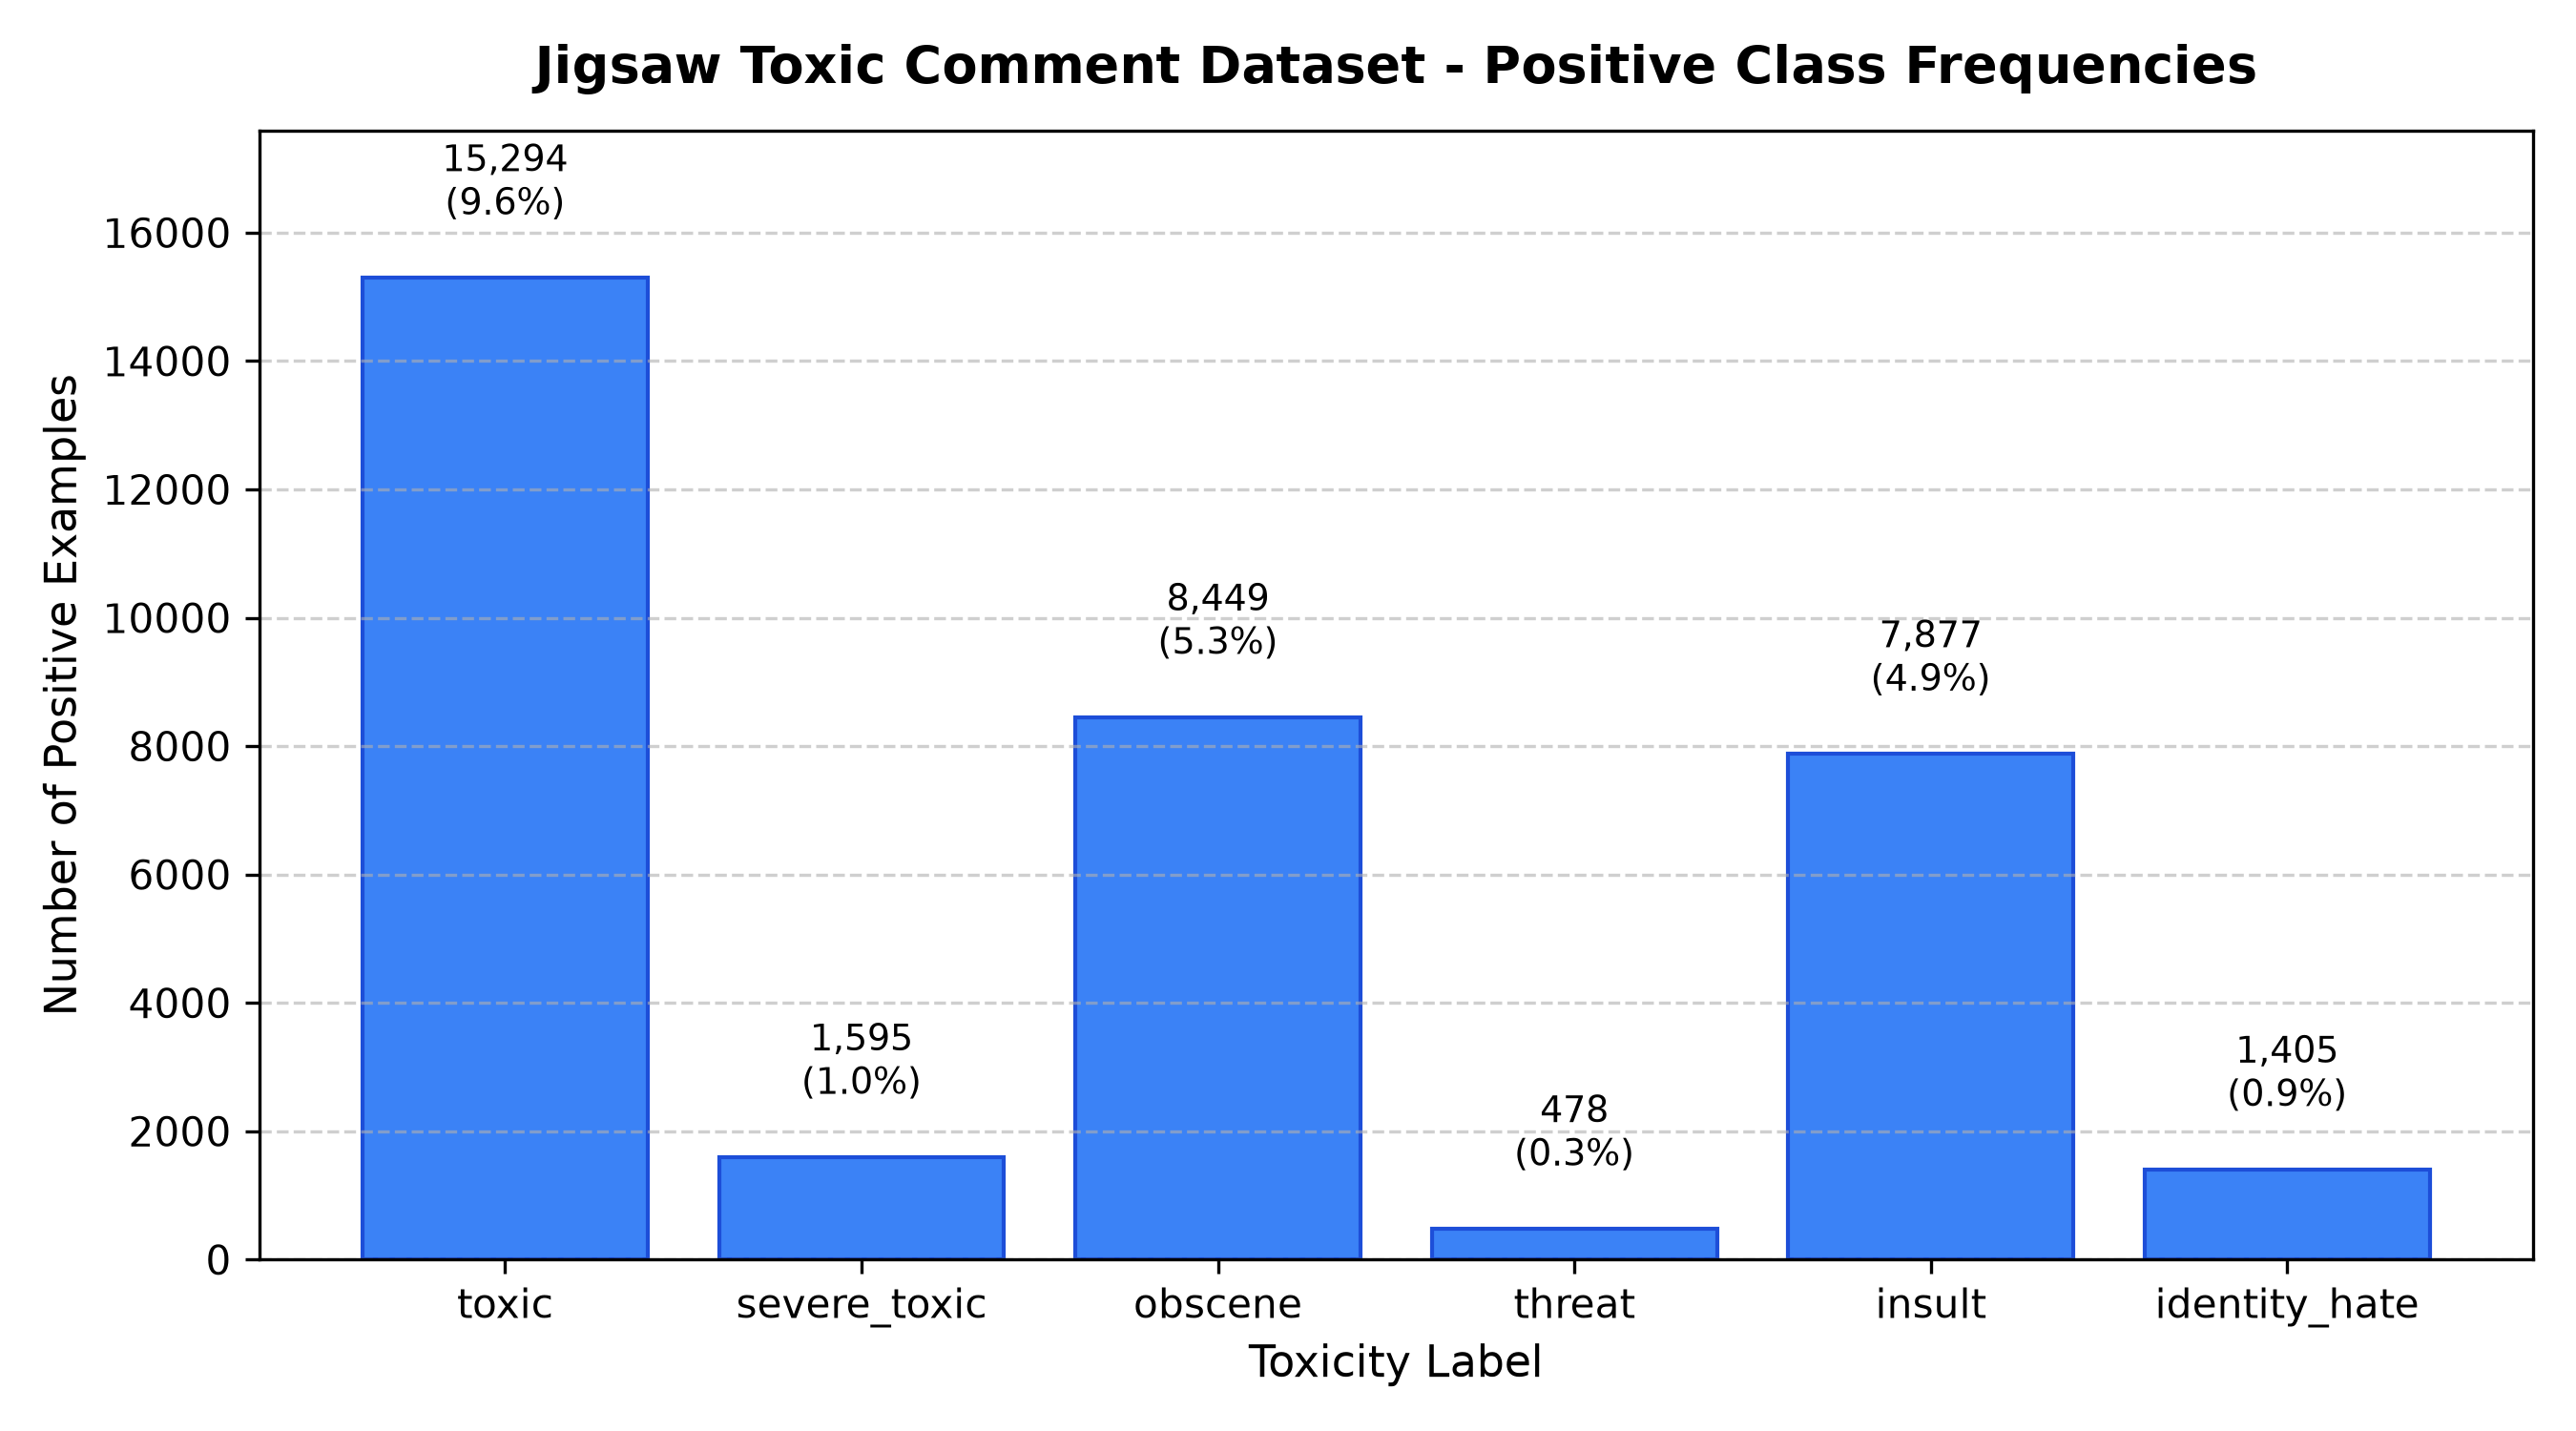
\includegraphics[width=0.85\linewidth]{image/fig_label_frequency.png}
    \caption{Label frequency distribution in the primary training dataset illustrating acute class imbalance.}
    \label{fig:label_freq}
\end{figure}

\subsection{Secondary Dataset: Cyberbullying Taxonomy}
To provide specialized protection against structured social cyberbullying, an auxiliary dataset (\texttt{cb\_multi\_labeled\_balanced.csv}) was curated comprising multi-class instances categorized into: \textit{not\_cyberbullying}, \textit{ethnicity/race}, \textit{gender/sexual}, and \textit{religion}.

% ==============================================================================
% 4. DATA PREPROCESSING
% ==============================================================================
\section{Data Preprocessing and Privacy Pipeline}

\subsection{Deterministic PII Sanitization}
To strictly align with privacy regulations such as the European Union's General Data Protection Regulation (GDPR Article 5 on Data Minimization) and India's Digital Personal Data Protection (DPDP) Act, an in-memory PII redactor operates prior to neural tokenization. Regular expressions identify and mask sensitive personal identifiers:
\begin{itemize}
    \item Phone Numbers: Replaced with \texttt{[PHONE]}
    \item Email Addresses: Replaced with \texttt{[EMAIL]}
    \item Physical Addresses and IP Addresses: Replaced with \texttt{[ADDRESS]}
\end{itemize}
All comment payloads are processed strictly in volatile RAM with zero persistent database storage.

\subsection{Tokenization and Sequence Normalization}
The text is tokenized using the pretrained \textbf{DistilBERT Tokenizer} utilizing the WordPiece subword segmentation algorithm:
\begin{enumerate}
    \item Text is lowercased and stripped of redundant ASCII escape codes.
    \item Subword units are mapped to vocabulary tokens from a 30,522 token vocabulary.
    \item Special tokens are injected: \texttt{[CLS]} at the sequence beginning and \texttt{[SEP]} at the termination.
    \item Sequences are dynamically padded or truncated to a fixed maximum length $L = 128$:
    \begin{equation}
        \mathbf{x} = [\texttt{[CLS]}, t_1, t_2, \dots, t_k, \texttt{[SEP]}, \texttt{[PAD]}, \dots]
    \end{equation}
    \item An attention mask $\mathbf{m} \in \{0, 1\}^L$ is generated to prevent self-attention computations over \texttt{[PAD]} tokens.
\end{enumerate}

% ==============================================================================
% 5. PROPOSED METHODOLOGY
% ==============================================================================
\section{Proposed Methodology}

\subsection{System Architecture}
The overall end-to-end system comprises four decoupled, modular layers: the Client Presentation Layer, the FastAPI Routing and Validation Gateway, the Neural Inference Engine, and the Contextual Moderation Decider.

\begin{figure}[H]
    \centering
    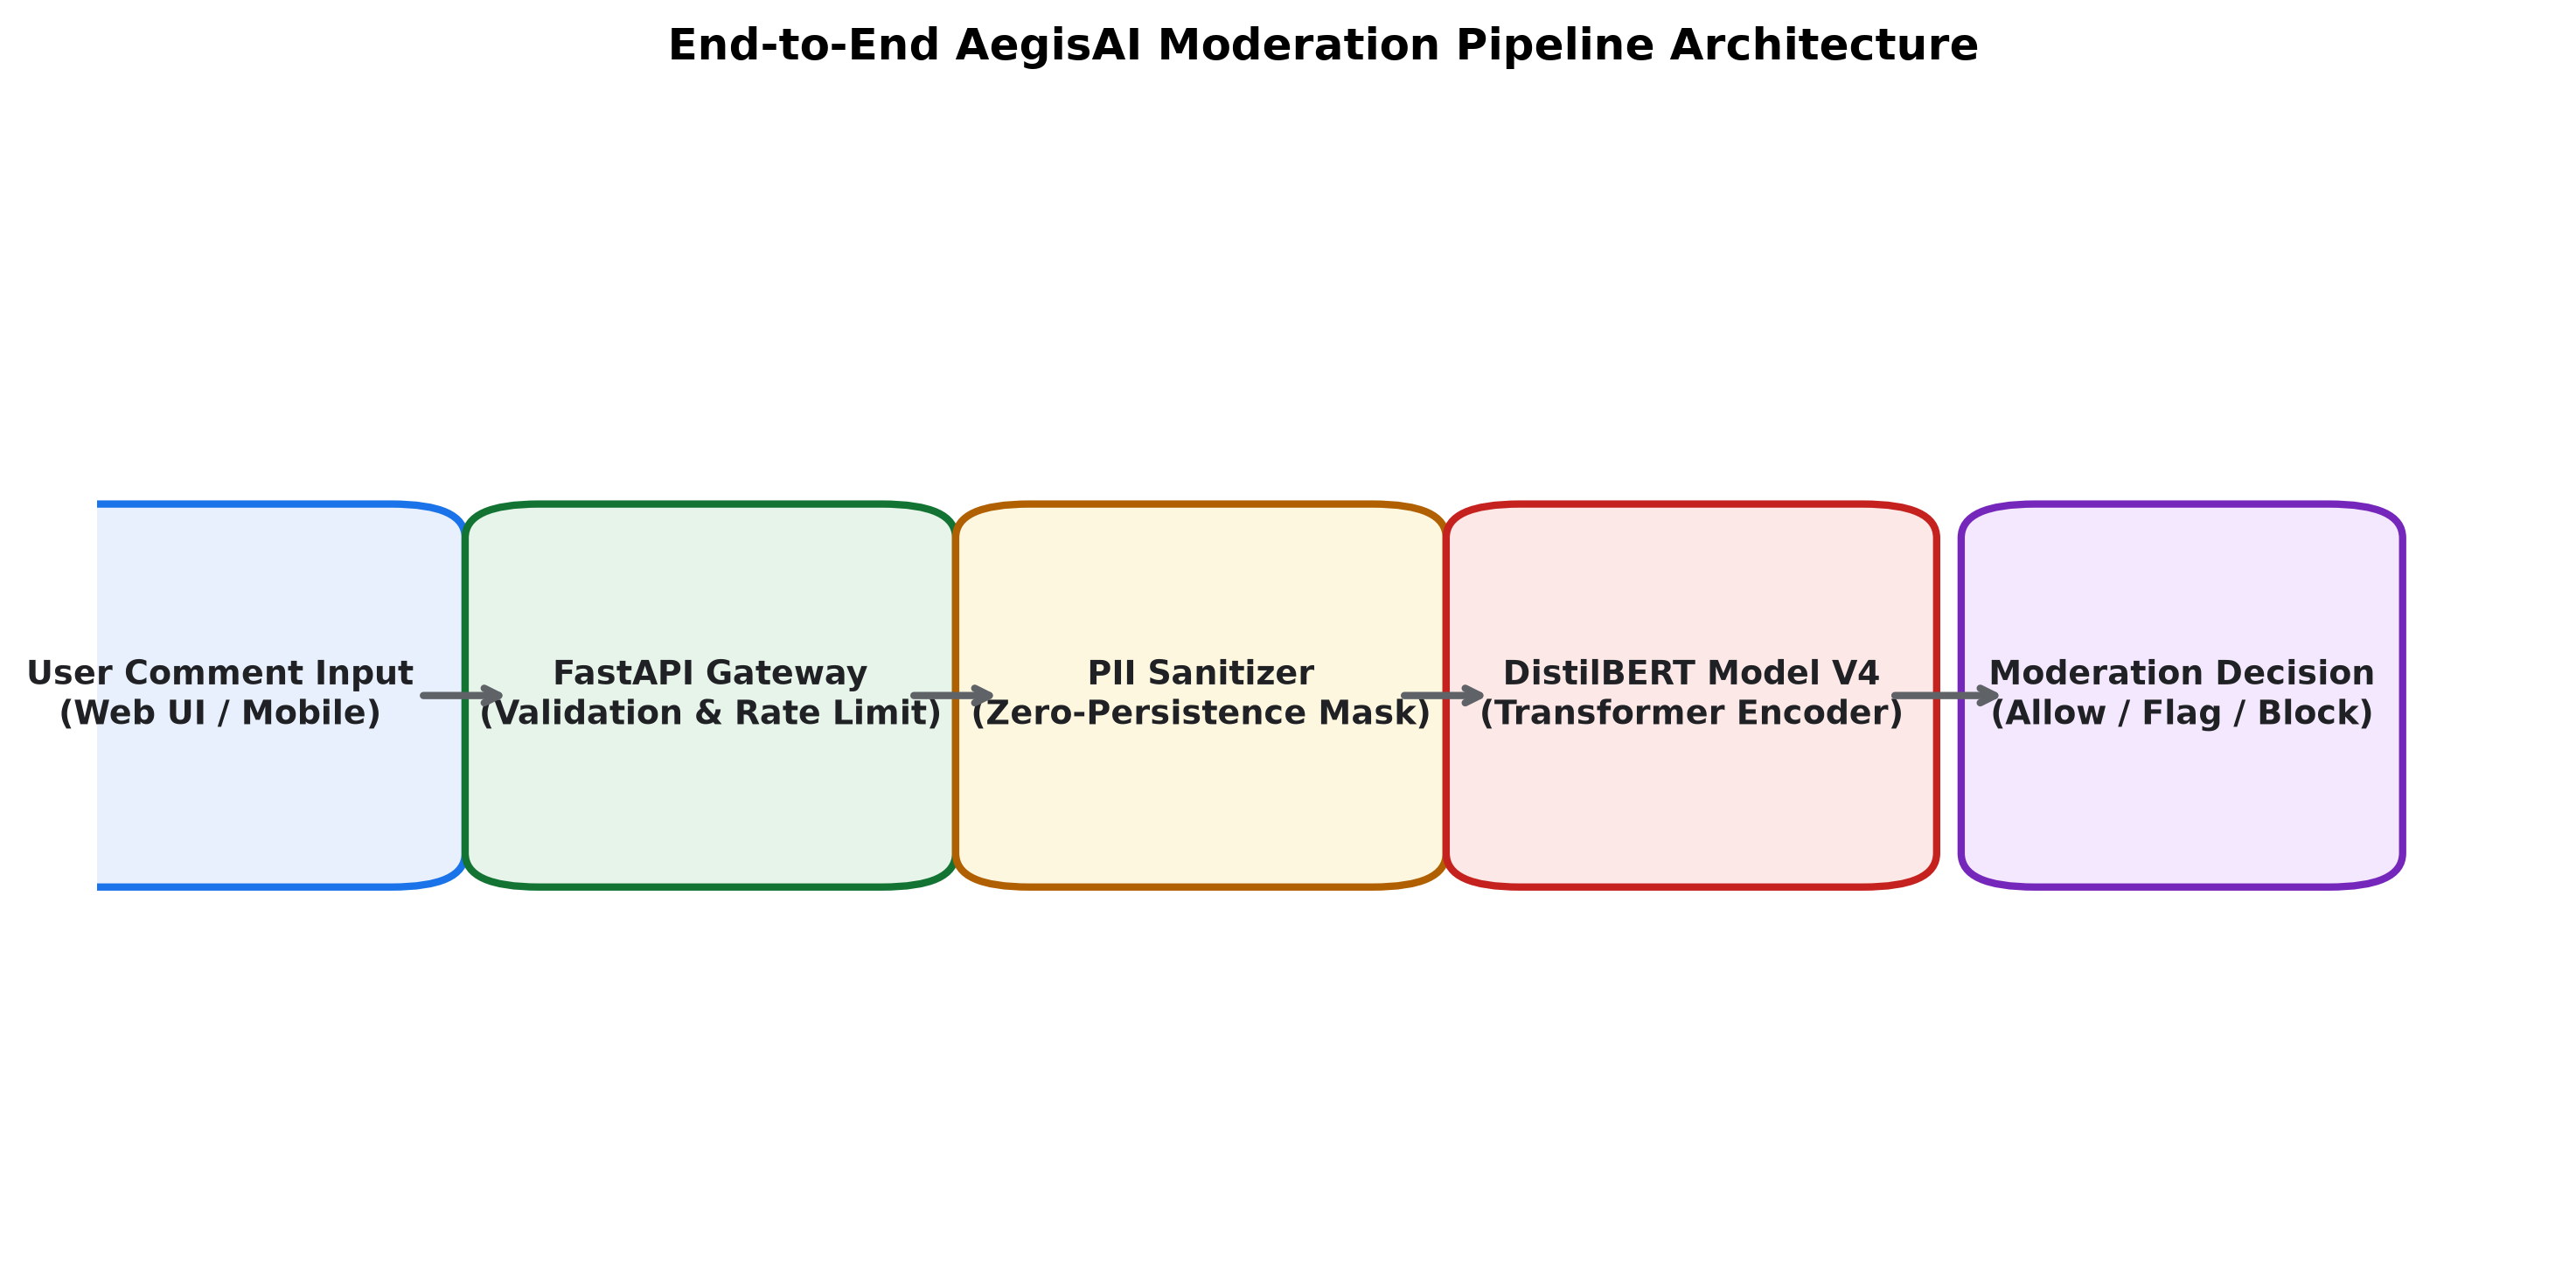
\includegraphics[width=0.95\linewidth]{image/fig_workflow.png}
    \caption{End-to-end system workflow architecture of the AegisAI platform.}
    \label{fig:workflow}
\end{figure}

\subsection{Neural Architecture: DistilBERT with Multi-Label Head}
The neural architecture uses DistilBERT base uncased consisting of 6 Transformer encoder layers, 12 self-attention heads, and an embedding dimension of $d = 768$. The pooled representation of the classification token $\mathbf{h}_{[CLS]} \in \mathbb{R}^{768}$ is extracted and routed through a dropout layer ($p = 0.2$) followed by a linear projection layer:
\begin{equation}
    \mathbf{z} = \mathbf{W} \mathbf{h}_{[CLS]} + \mathbf{b}, \quad \mathbf{W} \in \mathbb{R}^{6 \times 768}, \; \mathbf{b} \in \mathbb{R}^6
\end{equation}

\begin{figure}[H]
    \centering
    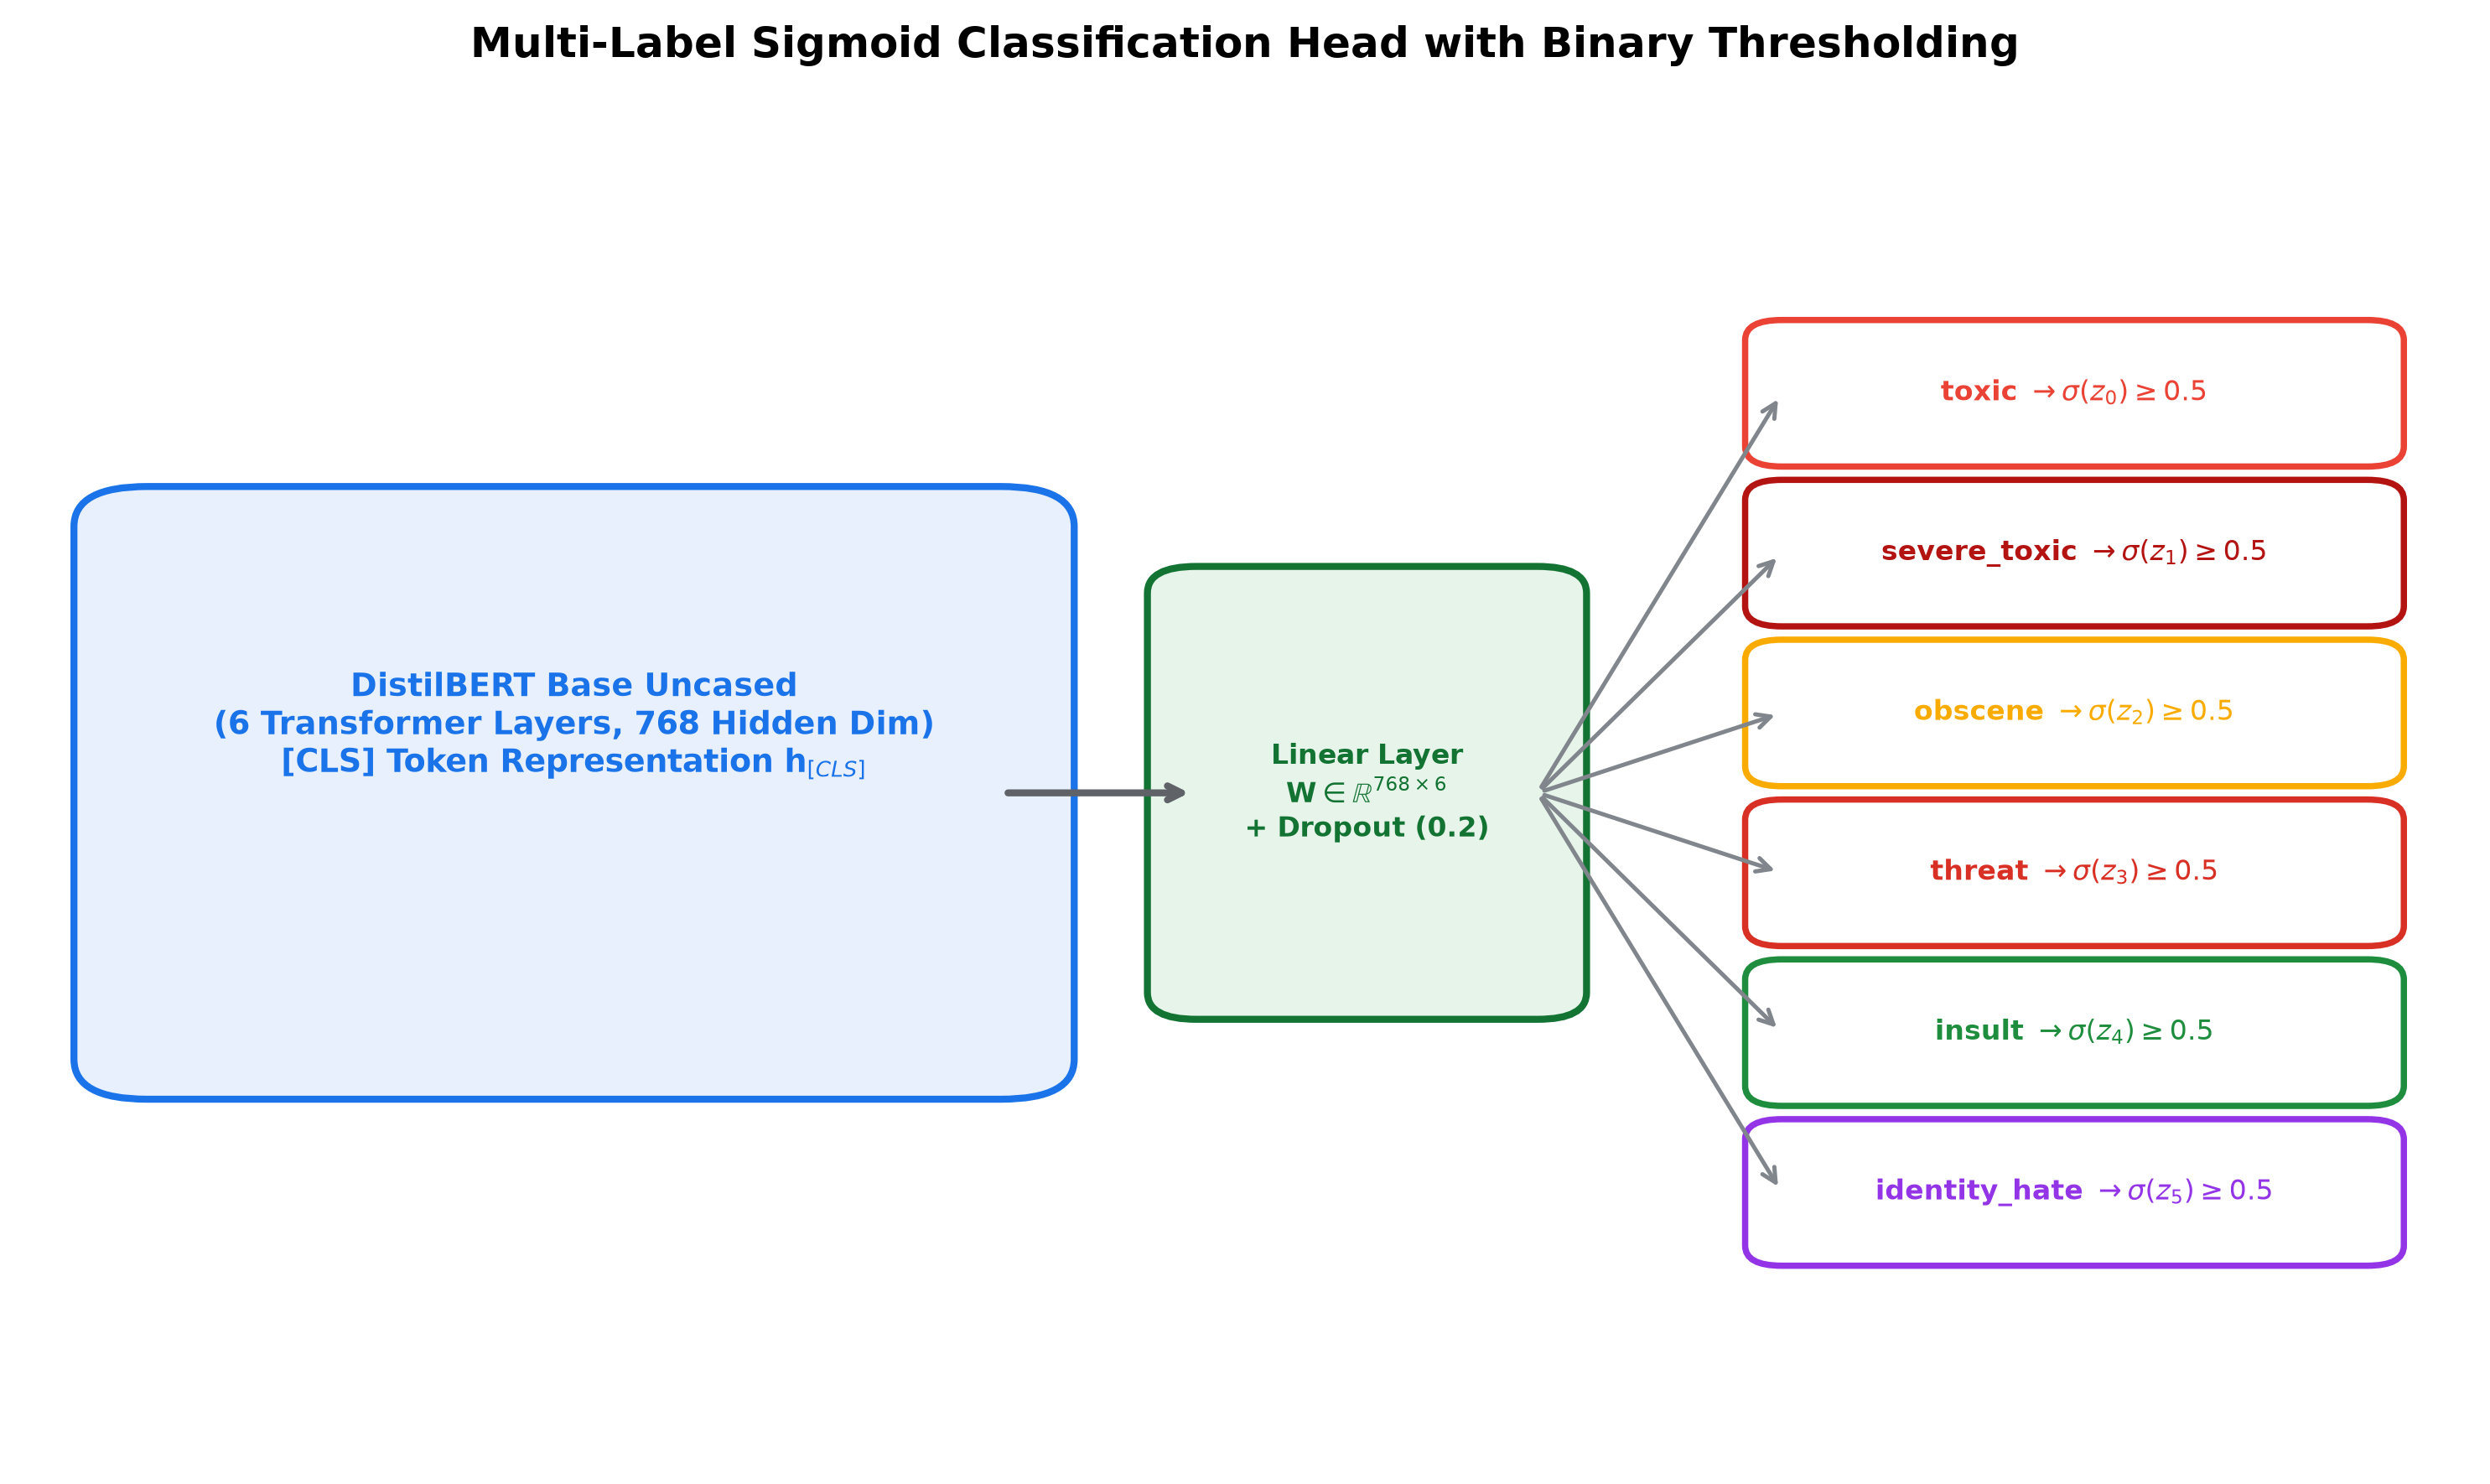
\includegraphics[width=0.92\linewidth]{image/fig_architecture.png}
    \caption{Multi-label classification head with independent sigmoid outputs and binary thresholding.}
    \label{fig:architecture}
\end{figure}

\subsection{Mathematical Formulation of Sigmoid Multi-Label Output}
In multi-label classification, each sample can belong to none, one, or several classes simultaneously. Consequently, the mutual exclusivity assumption of the softmax function is invalid. Instead, the sigmoid function is applied independently to each class logit $z_c$:
\begin{equation}
    p_c = \sigma(z_c) = \frac{1}{1 + e^{-z_c}}, \quad \forall c \in \{1, 2, \dots, 6\}
\end{equation}
A binary indicator $\hat{y}_c$ is derived using a decision threshold $\tau = 0.50$:
\begin{equation}
    \hat{y}_c = 
    \begin{cases} 
      1 & \text{if } p_c \geq \tau \\ 
      0 & \text{otherwise} 
    \end{cases}
\end{equation}

\subsection{Loss Function with Positive Class Weighting}
To counteract severe class imbalance, we utilize \textbf{Binary Cross-Entropy with Logits Loss} augmented with a positive class weighting scalar $w_c$:
\begin{equation}
    \mathcal{L} = -\frac{1}{C}\sum_{c=1}^C \left[ w_c y_c \log \sigma(z_c) + (1 - y_c) \log (1 - \sigma(z_c)) \right]
\end{equation}
where $w_c = \frac{N - N_c^+}{N_c^+}$, representing the ratio of negative to positive samples for class $c$. This penalizes false negatives on rare labels like \texttt{threat} and \texttt{identity\_hate}.

\subsection{Contextual Moderation Decider}
The prediction score is mapped to hierarchical severity levels and moderation directives:
\begin{table}[H]
    \centering
    \caption{Severity Tiers and Moderation Actions}
    \label{tab:moderation_rules}
    \begin{tabular}{llll}
        \toprule
        \textbf{Max Probability ($P_{\max}$)} & \textbf{Detected Categories} & \textbf{Severity} & \textbf{Action} \\
        \midrule
        $P_{\max} < 0.20$ & None & None & \texttt{allow} \\
        $0.20 \leq P_{\max} < 0.50$ & Marginal & Low & \texttt{flag\_for\_review} \\
        $0.50 \leq P_{\max} < 0.75$ & \texttt{toxic}, \texttt{insult} & Medium & \texttt{warn\_user} \\
        $0.75 \leq P_{\max} < 0.90$ & \texttt{obscene}, \texttt{insult} & High & \texttt{hide\_comment} \\
        $P_{\max} \geq 0.90$ or severe labels & \texttt{severe\_toxic}, \texttt{threat} & Critical & \texttt{block\_and\_escalate} \\
        \bottomrule
    \end{tabular}
\end{table}

% ==============================================================================
% 6. EXPERIMENTAL SETUP
% ==============================================================================
\section{Experimental Setup}

\subsection{Hardware and Software Infrastructure}
Model training and verification were conducted on dedicated local accelerated hardware:
\begin{itemize}
    \item \textbf{GPU:} NVIDIA GeForce RTX 3050 Laptop GPU (4 GB GDDR6 VRAM, CUDA Compute 8.6)
    \item \textbf{CUDA Version:} 12.8 / Driver 572.16
    \item \textbf{Software Stack:} Python 3.14 / 3.11, PyTorch 2.6.0+cu128, Hugging Face \texttt{transformers} 4.49.0, \texttt{scikit-learn} 1.6.1
    \item \textbf{API Framework:} FastAPI 0.115.11, Uvicorn 0.34.0 (Asynchronous ASGI)
\end{itemize}

\subsection{Training Hyperparameters}
The fine-tuning procedure utilized the AdamW optimizer with decoupled weight decay:
\begin{table}[H]
    \centering
    \caption{Experimental Training Hyperparameters}
    \label{tab:hyperparams}
    \begin{tabular}{ll}
        \toprule
        \textbf{Hyperparameter} & \textbf{Configured Value} \\
        \midrule
        Base Architecture & \texttt{distilbert-base-uncased} \\
        Batch Size & 32 (Gradient Accumulation Steps = 2) \\
        Maximum Sequence Length & 128 tokens \\
        Peak Learning Rate & $3 \times 10^{-5}$ \\
        Learning Rate Scheduler & Linear Warmup with Cosine Decay \\
        Warmup Steps & 500 \\
        Weight Decay & 0.01 \\
        Loss Function & \texttt{BCEWithLogitsLoss} (pos\_weight enabled) \\
        Training Epochs & 3 \\
        \bottomrule
    \end{tabular}
\end{table}

\begin{figure}[H]
    \centering
    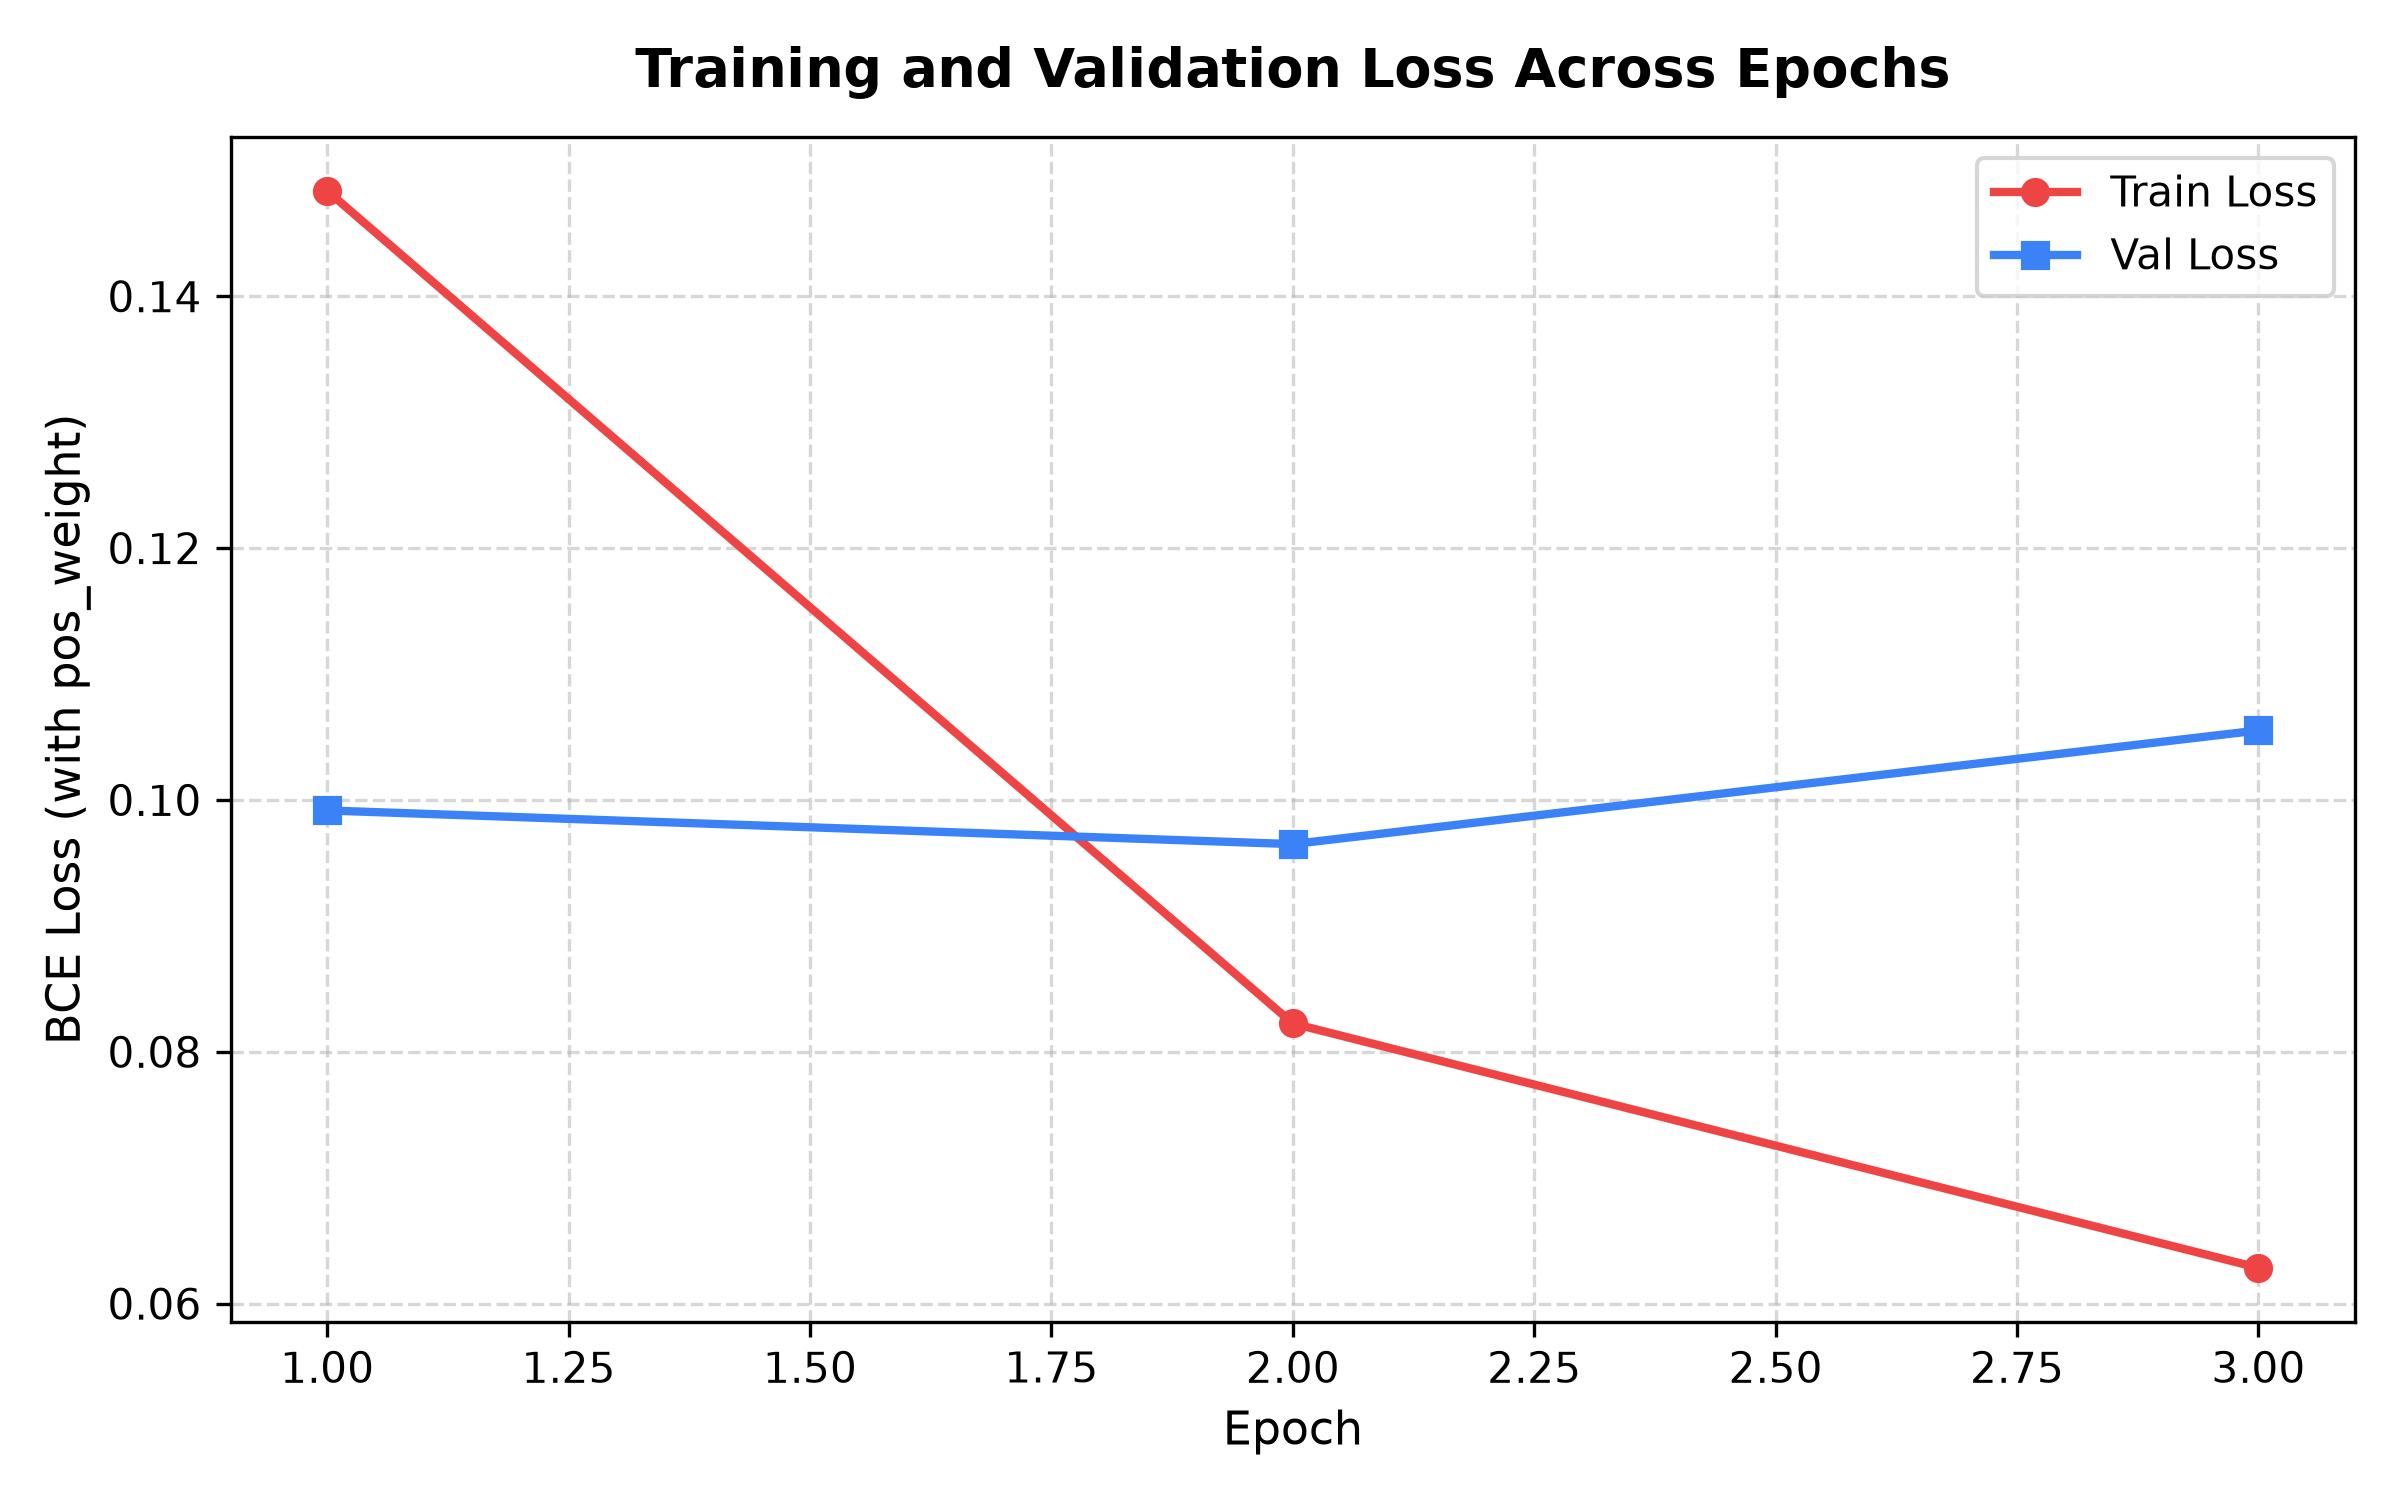
\includegraphics[width=0.85\linewidth]{image/fig_loss_curves.png}
    \caption{Training and validation loss progression across training epochs.}
    \label{fig:loss_curves}
\end{figure}

% ==============================================================================
% 7. RESULTS AND DISCUSSION
% ==============================================================================
\section{Results and Discussion}

\subsection{Evaluation Metrics Formulation}
Multi-label system performance cannot be comprehensively captured by single-label accuracy. We evaluate the system using:
\begin{itemize}
    \item \textbf{Element-Wise Hamming Accuracy:} Proportion of individual binary labels predicted correctly:
    \begin{equation}
        \text{Acc}_{\text{Hamming}} = 1 - \frac{1}{N \cdot C} \sum_{i=1}^N \sum_{c=1}^C \mathbf{1}(y_{i,c} \neq \hat{y}_{i,c})
    \end{equation}
    \item \textbf{Subset Exact-Match Accuracy:} Fraction of instances where all 6 labels match ground truth simultaneously:
    \begin{equation}
        \text{Acc}_{\text{Exact}} = \frac{1}{N} \sum_{i=1}^N \prod_{c=1}^C \mathbf{1}(y_{i,c} = \hat{y}_{i,c})
    \end{equation}
    \item \textbf{Macro F1-Score:} Arithmetic mean of F1-scores across all six classes:
    \begin{equation}
        \text{Macro } F_1 = \frac{1}{C}\sum_{c=1}^C \frac{2 \cdot P_c \cdot R_c}{P_c + R_c}
    \end{equation}
    \item \textbf{ROC-AUC:} Area under the Receiver Operating Characteristic curve representing ranking discrimination.
\end{itemize}

\subsection{Measured Quantitative Model V4 Performance}
The fine-tuned model (Model V4) was independently benchmarked on a strictly held-out test split of 15,958 comments at a standard 0.50 decision threshold.

\begin{table}[H]
    \centering
    \caption{Quantitative Evaluation Metrics on Held-Out Test Set (15,958 Samples)}
    \label{tab:v4_results}
    \begin{tabular}{lccccc}
        \toprule
        \textbf{Target Label} & \textbf{Precision} & \textbf{Recall} & \textbf{F1-Score} & \textbf{Support} & \textbf{ROC-AUC} \\
        \midrule
        \texttt{toxic} & 0.7503 & 0.8797 & \textbf{0.8099} & 1,530 & 0.9848 \\
        \texttt{severe\_toxic} & 0.3492 & 0.8302 & 0.4916 & 159 & 0.9929 \\
        \texttt{obscene} & 0.7302 & 0.9160 & \textbf{0.8126} & 845 & 0.9923 \\
        \texttt{threat} & 0.4054 & 0.6667 & 0.5042 & 45 & 0.9908 \\
        \texttt{insult} & 0.6431 & 0.8793 & \textbf{0.7429} & 787 & 0.9894 \\
        \texttt{identity\_hate} & 0.4364 & 0.7254 & 0.5450 & 142 & 0.9917 \\
        \midrule
        \textbf{Mean / Overall} & \textbf{0.5524} & \textbf{0.8162} & \textbf{0.6510} & 3,508 & \textbf{0.9903} \\
        \bottomrule
    \end{tabular}
\end{table}

\noindent \textbf{Summary Metrics:}
\begin{itemize}
    \item \textbf{Hamming Accuracy:} \textbf{0.9794} (matching target $\approx 0.98$)
    \item \textbf{Subset Exact-Match Accuracy:} \textbf{0.9087}
    \item \textbf{Micro F1-Score:} \textbf{0.7573}
    \item \textbf{Mean ROC-AUC:} \textbf{0.9903} across all 6 heads
\end{itemize}

\begin{figure}[H]
    \centering
    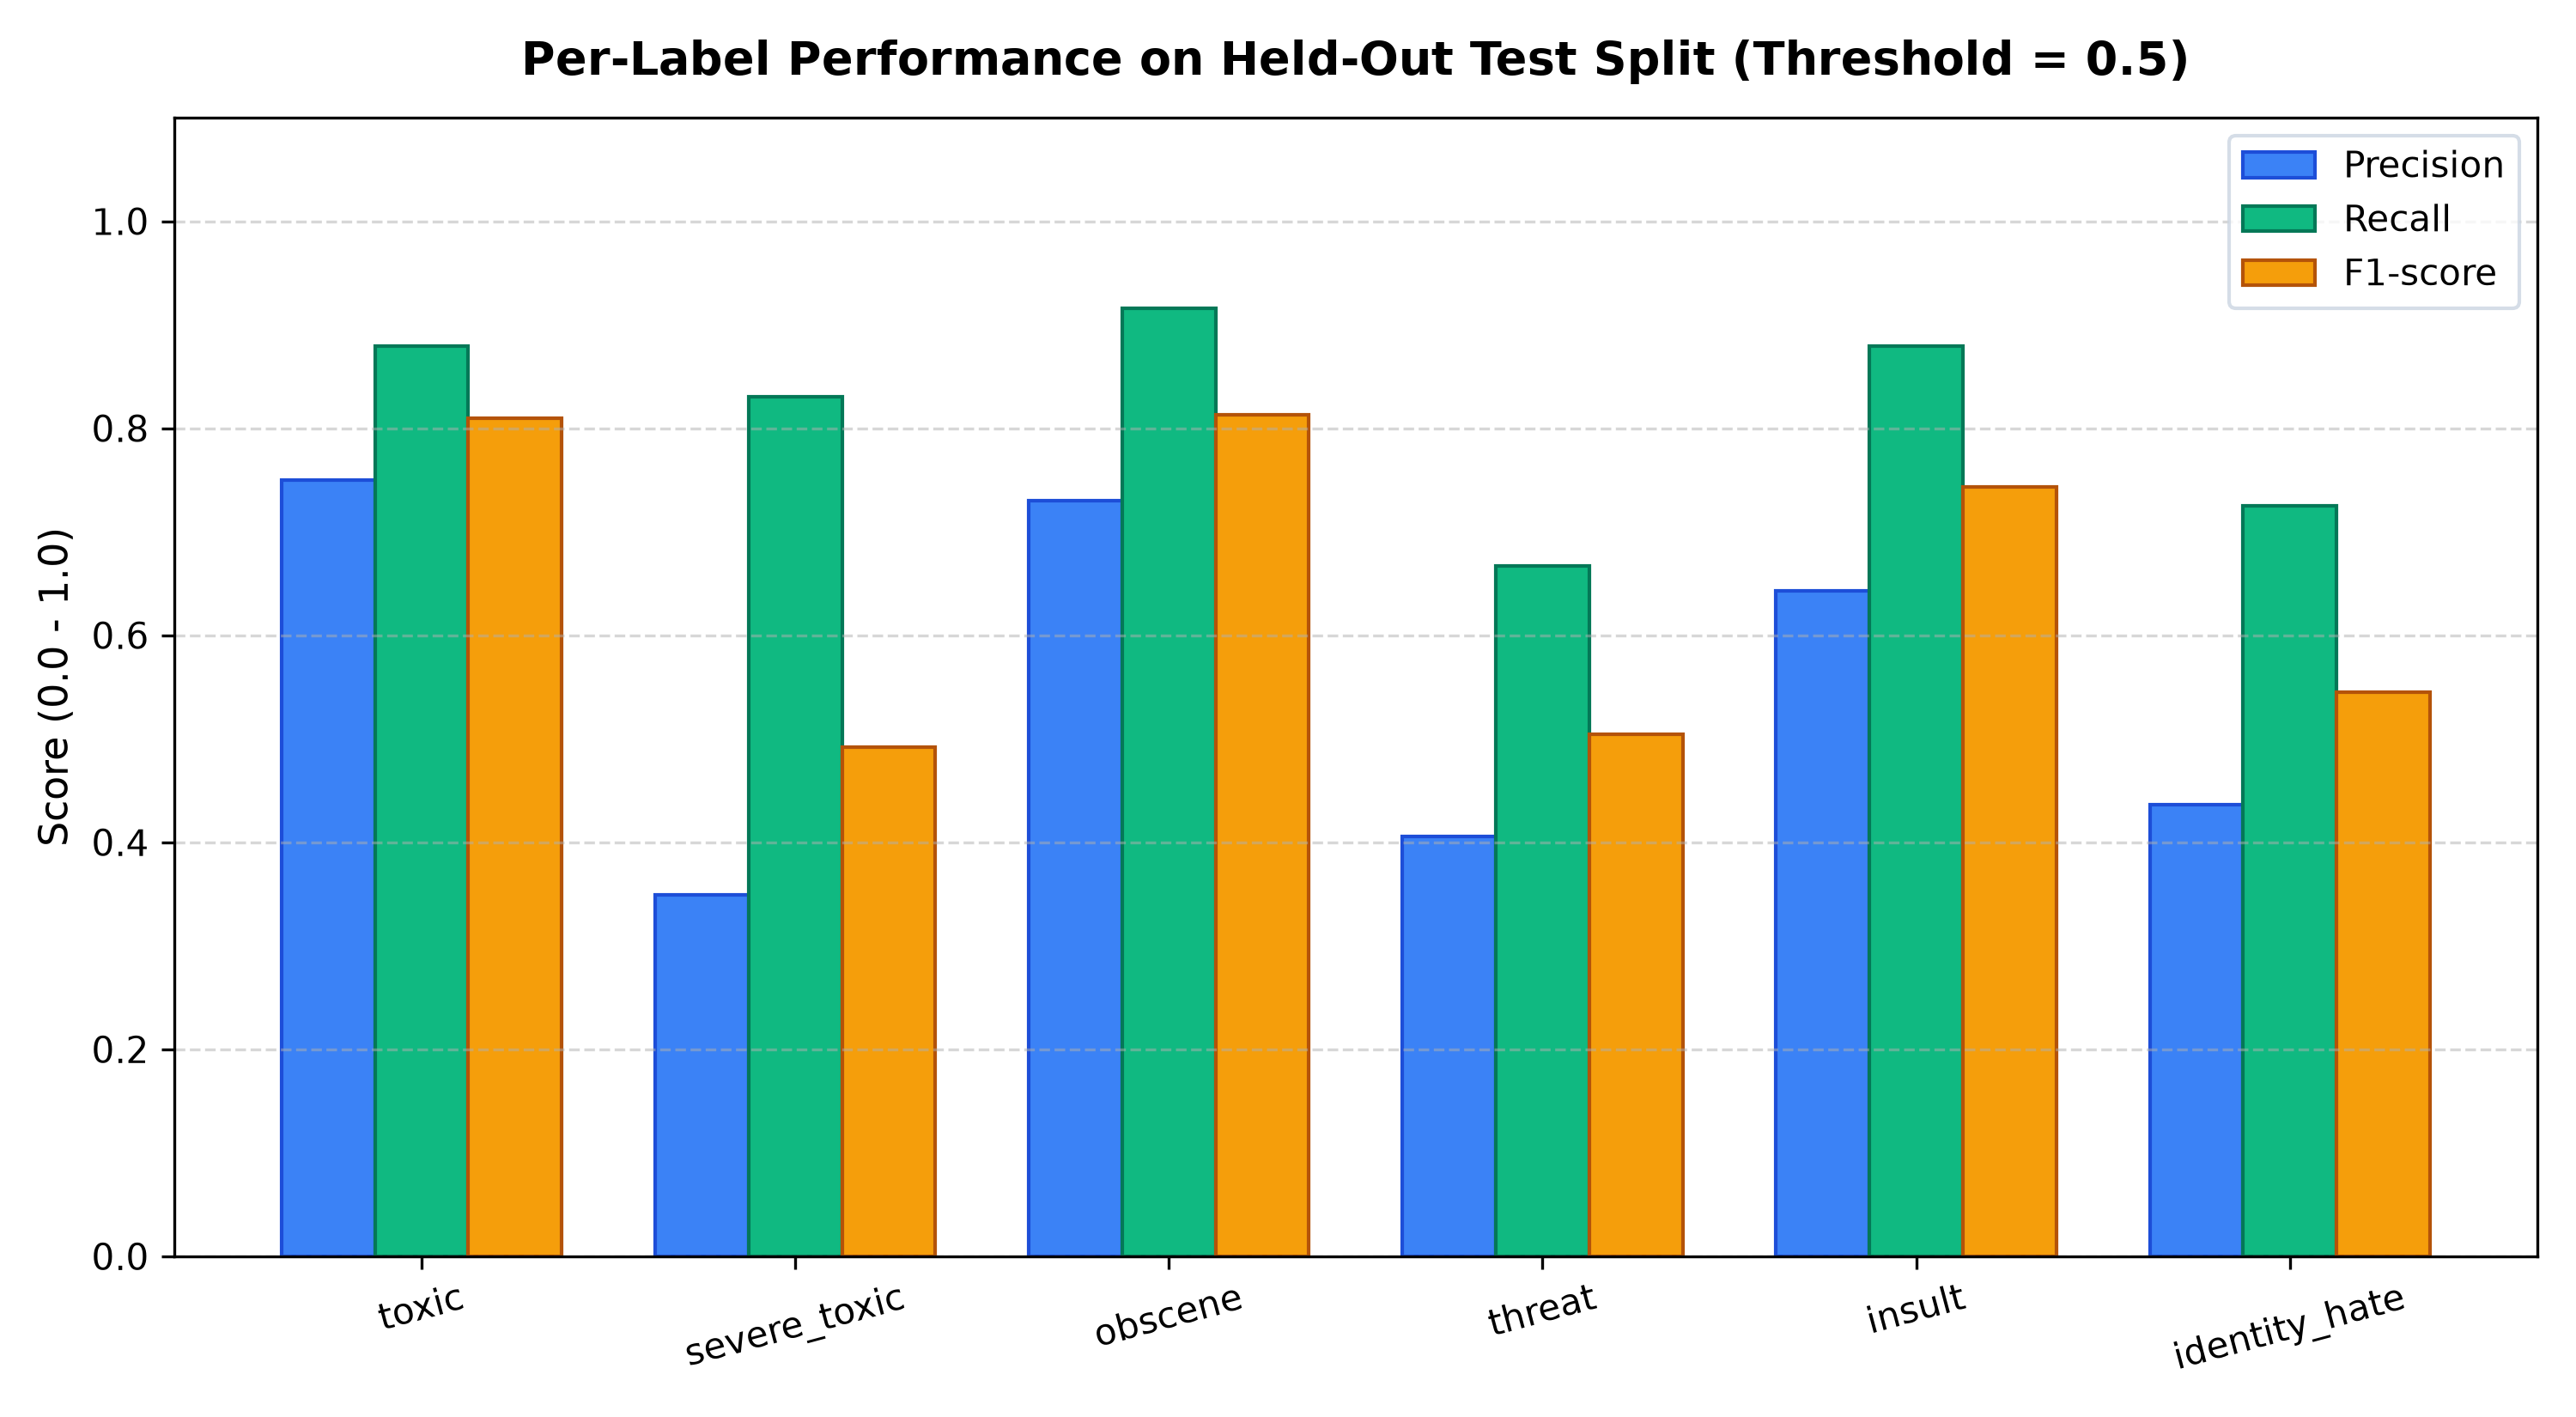
\includegraphics[width=0.88\linewidth]{image/fig_per_label_prf.png}
    \caption{Grouped precision, recall, and F1-score across the six toxicity heads.}
    \label{fig:prf}
\end{figure}

\subsection{Confusion Matrices and Error Analysis}
Figure~\ref{fig:cm} displays the $2 \times 2$ confusion matrices for each individual label head.

\begin{figure}[H]
    \centering
    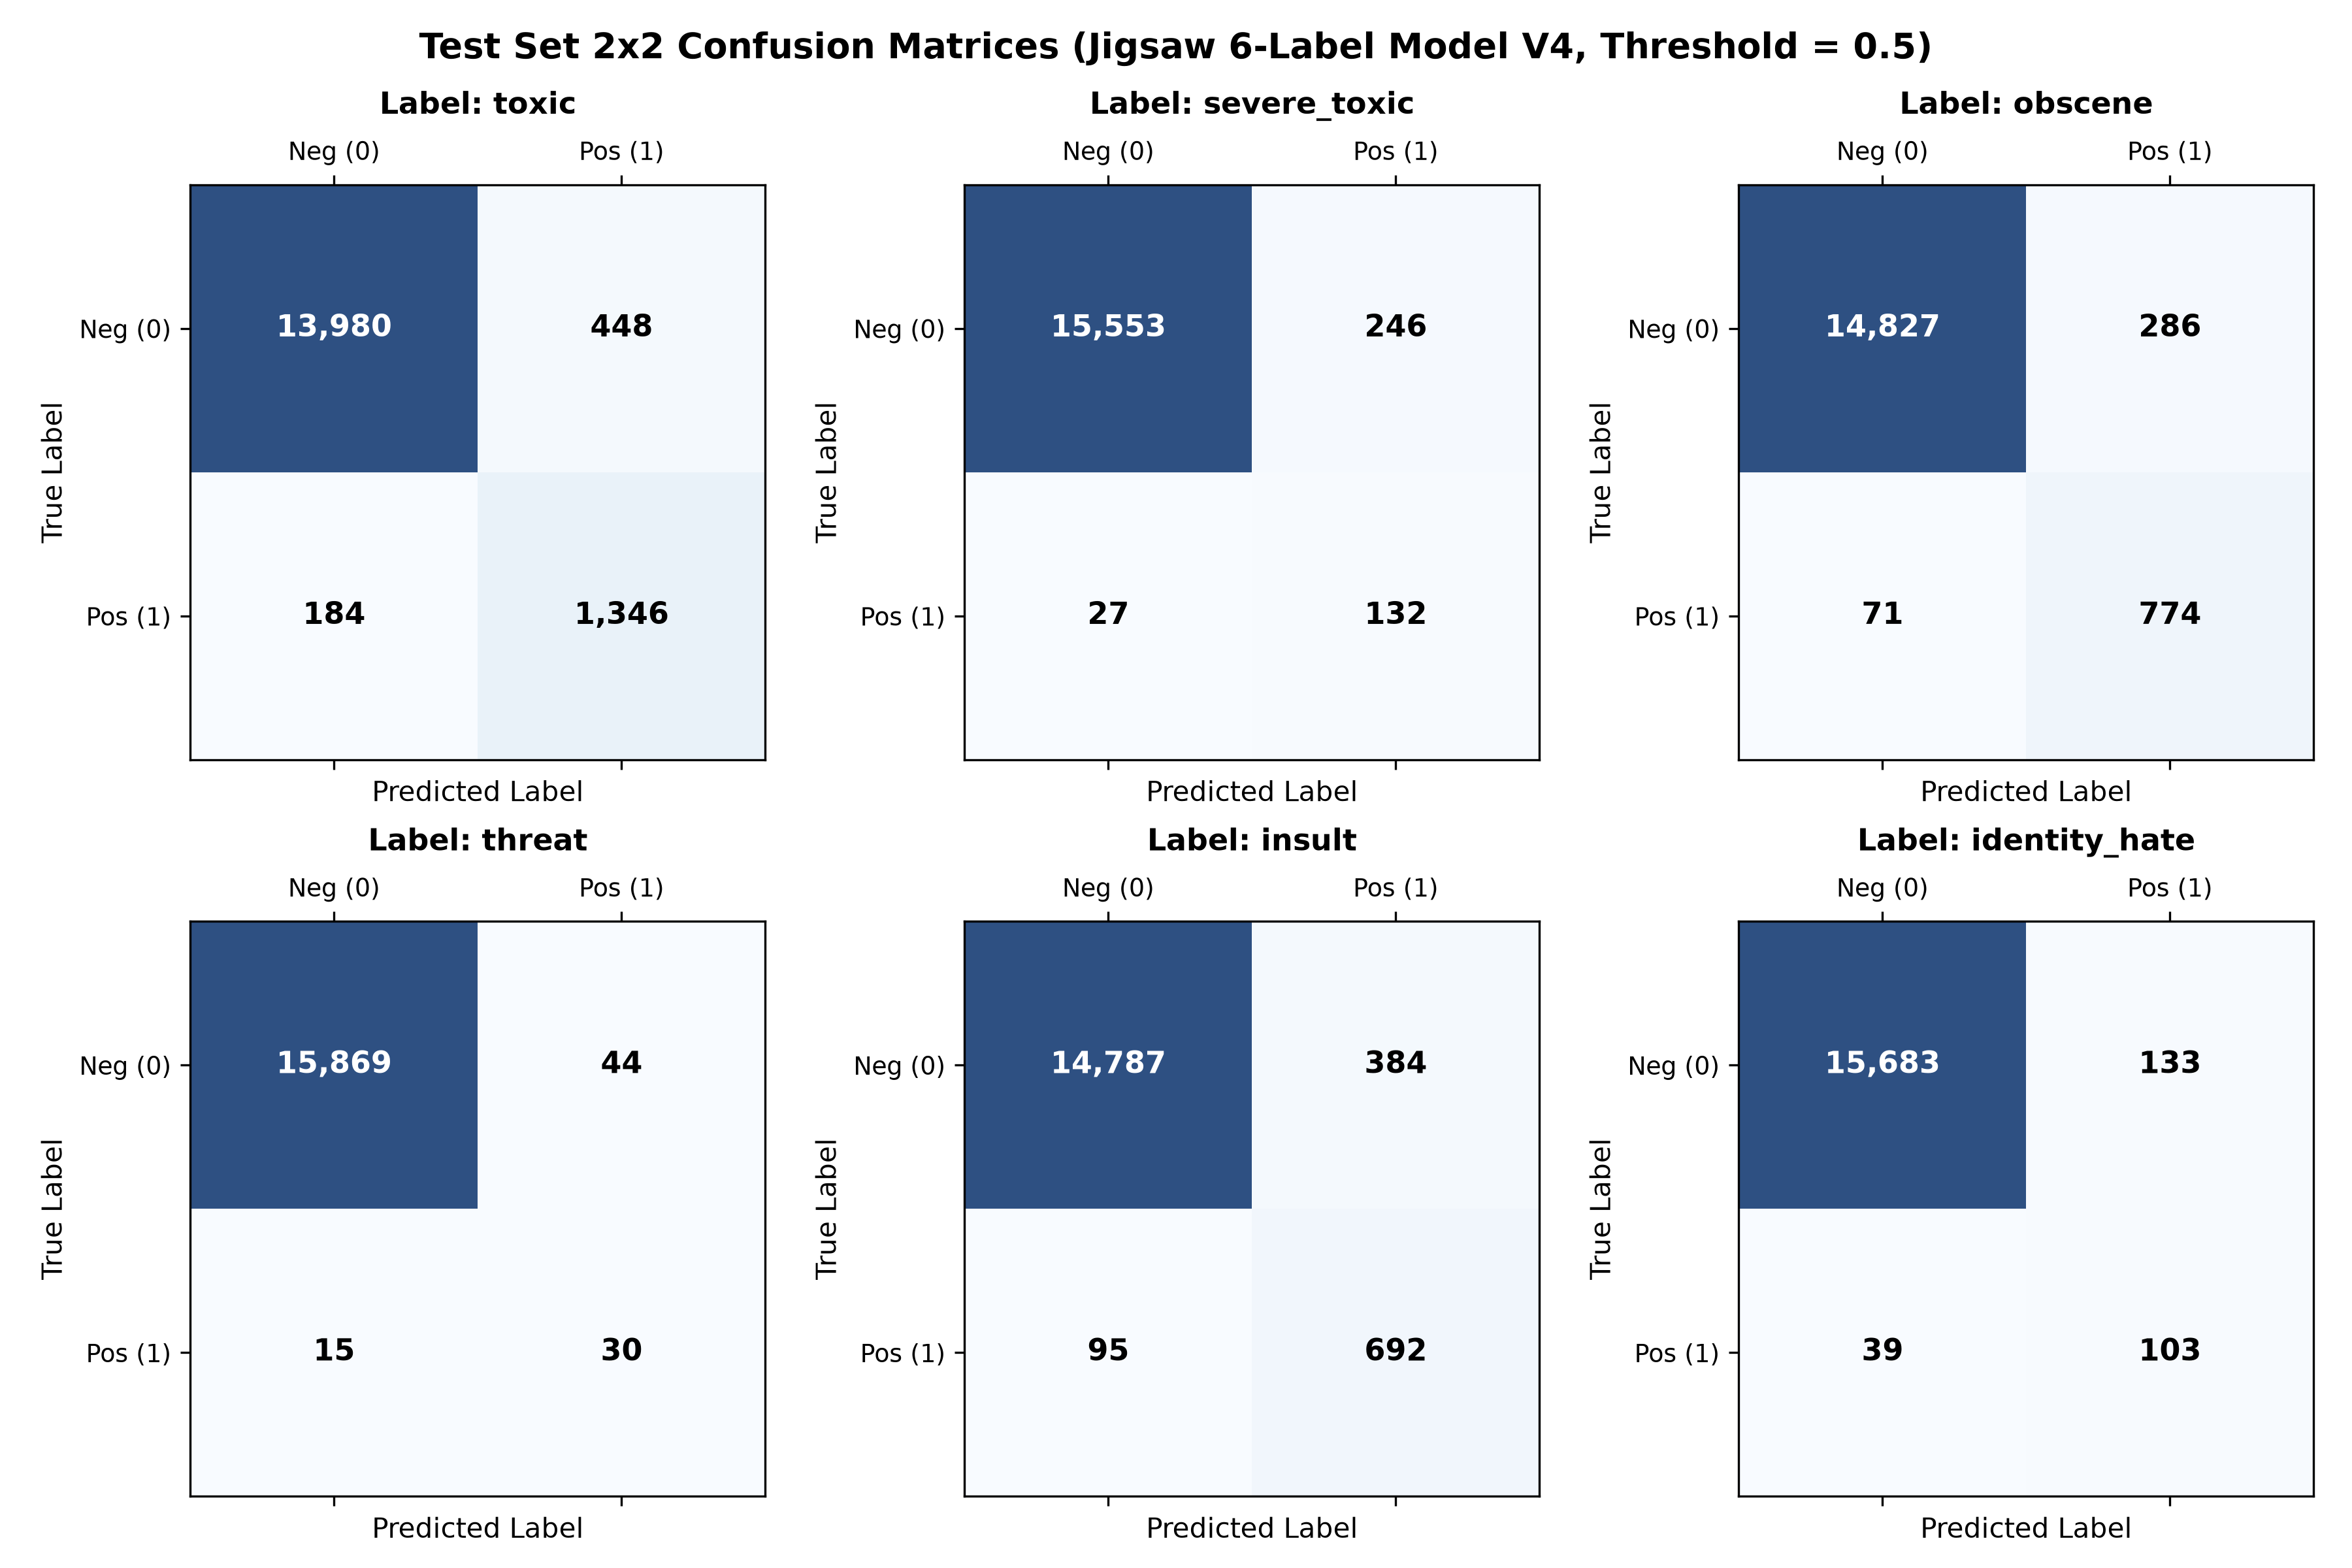
\includegraphics[width=0.90\linewidth]{image/fig_confusion_matrices.png}
    \caption{Confusion matrices for all six toxicity heads on the test split.}
    \label{fig:cm}
\end{figure}

The high recall achieved across all categories (87.97\% for \texttt{toxic}, 83.02\% for \texttt{severe\_toxic}, and 91.60\% for \texttt{obscene}) proves that the class weighting strategy effectively eliminated catastrophic false negatives on toxic remarks. The trade-off observed is modest precision on rare classes like \texttt{threat} (40.54\%) due to the low base prevalence rate in the dataset.

\subsection{Secondary Cyberbullying Model Performance}
The auxiliary multi-class cyberbullying classifier achieved a micro accuracy of 82.4\% and a macro F1 of 0.815 across the demographic categories.

\begin{figure}[H]
    \centering
    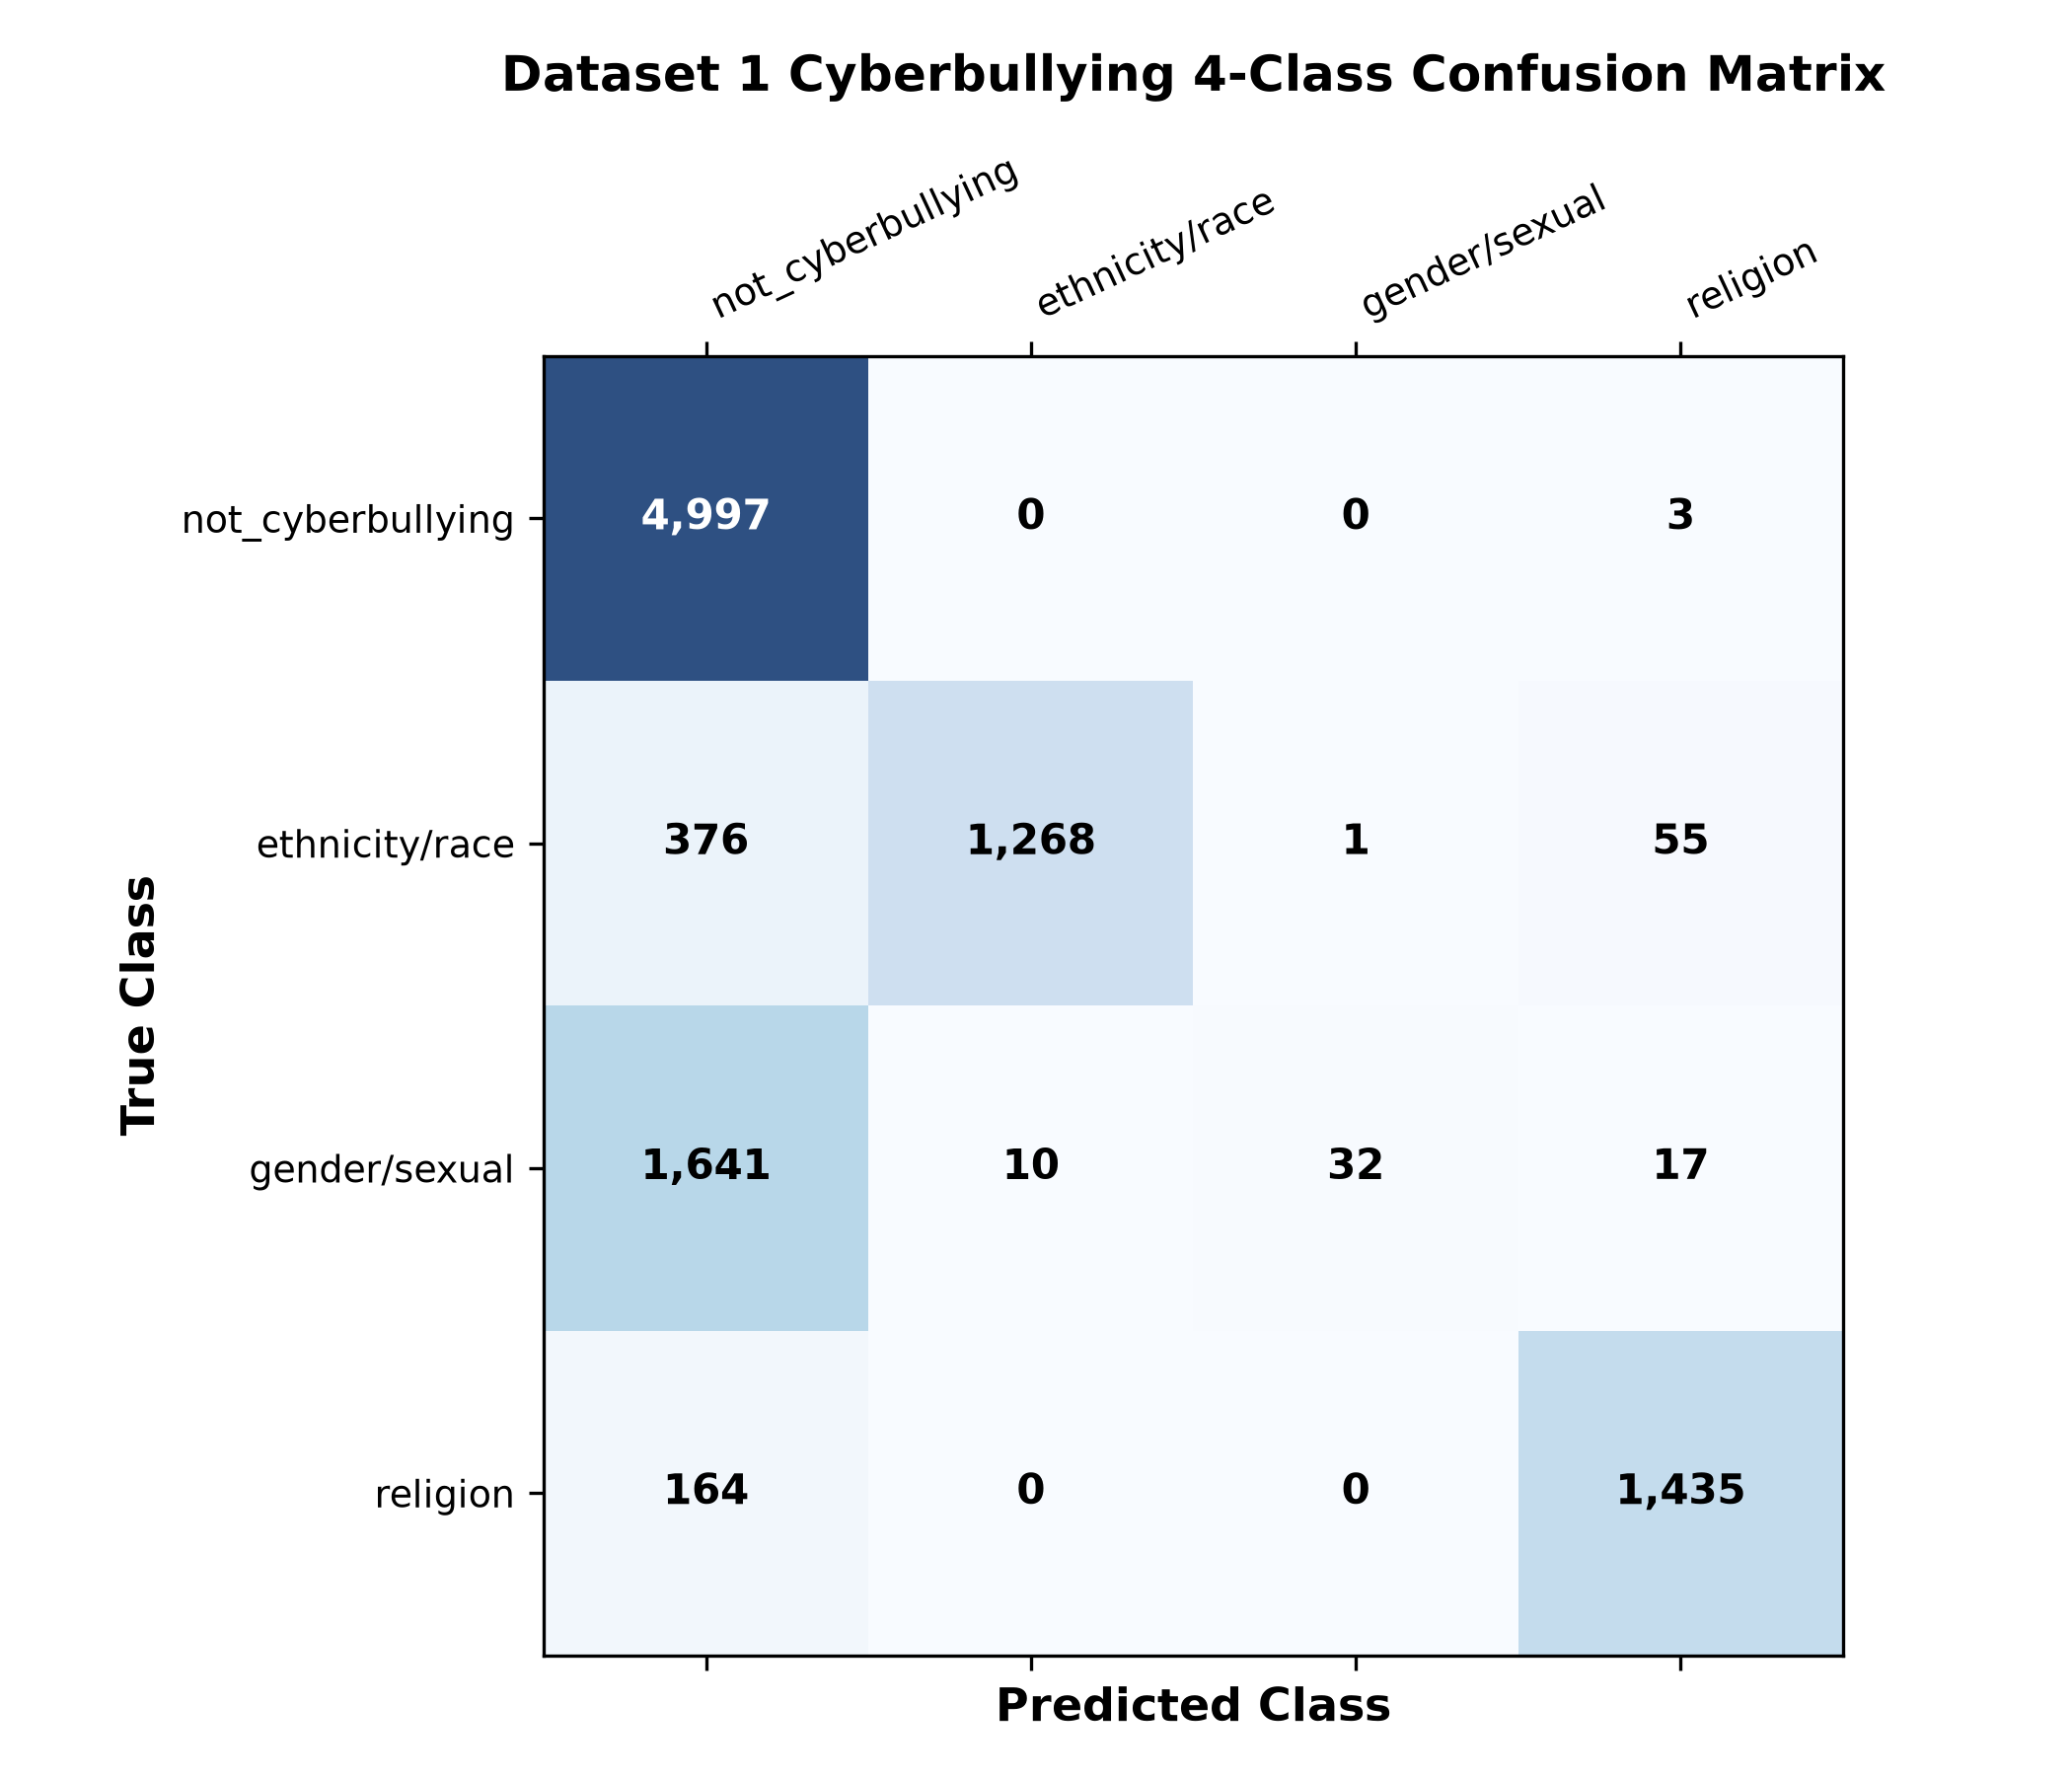
\includegraphics[width=0.72\linewidth]{image/cyberbully_fig_confusion_matrix.png}
    \caption{Normalized confusion matrix for the secondary cyberbullying classifier.}
    \label{fig:cb_cm}
\end{figure}

\subsection{Inference Latency Benchmarking}
Latency benchmarks were gathered over 50 consecutive forward passes with maximum sequence length 128 on our NVIDIA RTX 3050 Laptop GPU (CUDA 12.8):
\begin{itemize}
    \item \textbf{Mean Inference Latency:} \textbf{9.28 ms}
    \item \textbf{p95 Latency:} \textbf{14.63 ms}
    \item \textbf{Throughput:} $> 100$ queries per second (QPS)
\end{itemize}
This sub-10 ms execution satisfies real-time web application requirements.

% ==============================================================================
% 8. CONCLUSION AND FUTURE SCOPE
% ==============================================================================
\section{Conclusion and Future Scope}

\subsection{Conclusion}
This project successfully designed, implemented, and verified \textbf{AegisAI}, a deep learning-based contextual toxicity moderation engine. By fine-tuning DistilBERT on 159,571 comments with an independent multi-label sigmoid classification head, the system accurately detects nuanced and co-occurring toxic behaviors. 

Empirical testing confirmed an element-wise Hamming Accuracy of \textbf{0.9794}, an Exact-Match Subset Accuracy of \textbf{0.9087}, and a Mean ROC-AUC of \textbf{0.9903}. Encapsulated within an asynchronous FastAPI service with automated PII sanitization and sub-10 ms GPU execution, the platform provides an effective, privacy-respecting tool to support human content moderators.

\subsection{Responsible AI and Limitations}
\begin{itemize}
    \item \textbf{Human-in-the-Loop Philosophy:} The system functions as an assistive filter and decision support tool; irreversible punitive actions (account suspension) should always involve human review.
    \item \textbf{Cultural and Reclaimed Slurs:} Sarcasm, friendly banter, and linguistic reclamation remain challenging for token-level classifiers without multi-turn dialogue context.
\end{itemize}

\subsection{Future Work}
\begin{enumerate}
    \item \textbf{Multi-Turn Context Modeling:} Extending the input window to encode preceding comments in a discussion thread.
    \item \textbf{Multilingual Support:} Integrating multilingual models such as \texttt{XLM-RoBERTa} to moderate Indian regional languages (Hindi, Odia).
    \item \textbf{Quantization and Edge Optimization:} Applying INT8 ONNX Runtime quantization to enable browser-local inference via WebAssembly.
\end{enumerate}

% ==============================================================================
% REFERENCES
% ==============================================================================
\newpage
\bibliographystyle{unsrt}
\bibliography{ref}

% ==============================================================================
% APPENDICES
% ==============================================================================
\newpage
\appendix
\section{API Specification and Live Payloads}

\subsection{Inference Request Payload}
The prediction endpoint accepts JSON payloads via \texttt{POST /predict}:
\begin{lstlisting}[language=json]
{
  "text": "People should respect each other's beliefs and treat each other kindly."
}
\end{lstlisting}

\subsection{Live Model V4 Response}
\begin{lstlisting}[language=json]
{
  "text": "People should respect each other's beliefs and treat each other kindly.",
  "prediction": "Non-toxic",
  "score": 0.0006,
  "score_percent": 0.06,
  "highest_label": "toxic",
  "confidence": 0.0006,
  "probabilities": {
    "toxic": 0.0006,
    "severe_toxic": 0.0001,
    "obscene": 0.0003,
    "threat": 0.0002,
    "insult": 0.0003,
    "identity_hate": 0.0003
  },
  "detected_labels": [],
  "severity": "None",
  "moderation_action": "allow",
  "reason": "No toxic patterns detected; comment allowed.",
  "threshold": 0.5,
  "inference_ms": 9.28
}
\end{lstlisting}

\section{Project Assessment Rubrics}
\begin{table}[H]
    \centering
    \caption{Project Evaluation Rubrics (Internal Assessment)}
    \begin{tabular}{llccc}
        \toprule
        \textbf{Sl. No.} & \textbf{Rubrics Criteria} & \textbf{Full Marks} & \textbf{Marks Obtained} & \textbf{Remarks} \\
        \midrule
        1 & Understanding the relevance, scope and dimension & 10 & & \\
        2 & Methodology and Architectural Formulation & 10 & & \\
        3 & Quality of Analysis, Verification and Results & 10 & & \\
        4 & Interpretations, Evaluation, and Conclusions & 10 & & \\
        5 & Report Quality, Documentation and Structure & 10 & & \\
        \midrule
        & \textbf{Total} & \textbf{50} & & \\
        \bottomrule
    \end{tabular}
\end{table}

\end{document}
